\section{Examples of spin models}

\subsection{2-state,2-spin system}\label{sec:2spin_2states}

Consider a two-spin system and a corresponding complete model. Then, there are 4 different configurations that can be observed and, including $\phi^0$, there are 4 spin operators.
The probability for the 4 different configurations can be written as

\begin{align*}
    p(s_1=1, s_2=1) &= \frac{1}{Z(\mathbf{g})} e^{g_0 \phi^0(s_1=1, s_2=1) + g_1 \phi^1(s_1=1, s_2=1) + g_2 \phi^2(s_1=1, s_2=1) + g_3 \phi^3(s_1=1, s_2=1)},\\
    p(s_1=-1, s_2=1) &= \frac{1}{Z(\mathbf{g})} e^{g_0 \phi^0(s_1=-1, s_2=1) + g_1 \phi^1(s_1=-1, s_2=1) + g_2 \phi^2(s_1=-1, s_2=1) + g_3 \phi^3(s_1=-1, s_2=1)},\\
    p(s_1=1, s_2=-1) &= \frac{1}{Z(\mathbf{g})} e^{g_0 \phi^0(s_1=1, s_2=-1) + g_1 \phi^1(s_1=1, s_2=-1) + g_2 \phi^2(s_1=1, s_2=-1) + g_3 \phi^3(s_1=1, s_2=-1)},\\
    p(s_1=-1, s_2=-1) &= \frac{1}{Z(\mathbf{g})} e^{g_0 \phi^0(s_1=-1, s_2=-1) + g_1 \phi^1(s_1=-1, s_2=-1) + g_2 \phi^2(s_1=-1, s_2=-1) + g_3 \phi^3(s_1=-1, s_2=-1)},\\
\end{align*}

\noindent
which can be rewritten as

\begin{align*}
    p(s_1=1, s_2=1) &= \frac{1}{Z(\mathbf{g})} e^{g_0 + g_1 + g_2 + g_3},\\
    p(s_1=-1, s_2=1) &= \frac{1}{Z(\mathbf{g})} e^{g_0 - g_1 + g_2 - g_3},\\
    p(s_1=1, s_2=-1) &= \frac{1}{Z(\mathbf{g})} e^{g_0 + g_1 - g_2 - g_3},\\
    p(s_1=-1, s_2=-1) &= \frac{1}{Z(\mathbf{g})} e^{g_0 - g_1 - g_2 + g_3}.
\end{align*}

\noindent
In case of a complete model, we can define a spin operator matrix,

\begin{equation}
    \mathbf{S}^{(2)} = \begin{bmatrix}
        \phi^0(s=1) & \phi^1(s=1)\\
        \phi^0(s=-1) & \phi^1(s=-1)
    \end{bmatrix} = \begin{bmatrix}
        1 & 1\\
        1 & -1
    \end{bmatrix},
\end{equation}

\noindent
such that the probability of a configuration can be written as an element of the matrix vector product,

\begin{equation}\label{eq:relation_p_g}
    \mathbf{p} = \exp\left(\bigotimes_{i = 1}^{n} \mathbf{S}^{(2)} \cdot \mathbf{g}\right).
\end{equation}

\noindent
In a two-spin system, the matrix $\bigotimes_{i = 1}^{n} \mathbf{S}^{(2)}$ is equal to

\begin{align*}
    \scriptstyle
    \mathbf{S}^{(2)} \otimes \mathbf{S}^{(2)} &= \begin{bmatrix}
        \phi^0(s_2=1) & \phi^1(s_2=1)\\
        \phi^0(s_2=-1) & \phi^1(s_2=-1)
    \end{bmatrix} \otimes \begin{bmatrix}
        \phi^0(s_1=1) & \phi^1(s_1=1)\\
        \phi^0(s_1=-1) & \phi^1(s_1=-1)
    \end{bmatrix}\\
    &= \begin{bmatrix}
        \scriptstyle \phi^0(s_2=1) \phi^0(s_1=1) & \scriptstyle \phi^0(s_2=1) \phi^1(s_1=1) & \scriptstyle \phi^1(s_2=1) \phi^0(s_1=1) & \scriptstyle \phi^1(s_2=1) \phi^1(s_1=1)\\
        \scriptstyle \phi^0(s_2=1) \phi^0(s_1=-1) & \scriptstyle \phi^0(s_2=1) \phi^1(s_1=-1) & \scriptstyle \phi^1(s_2=1) \phi^0(s_1=-1) & \scriptstyle \phi^1(s_2=1) \phi^1(s_1=-1)\\
        \scriptstyle \phi^0(s_2=-1) \phi^0(s_1=1) & \scriptstyle \phi^0(s_2=-1) \phi^1(s_1=1) & \scriptstyle \phi^1(s_2=-1) \phi^0(s_1=1) & \scriptstyle \phi^1(s_2=-1) \phi^1(s_1=1)\\
        \scriptstyle \phi^0(s_2=-1) \phi^0(s_1=-1) & \scriptstyle \phi^0(s_2=-1) \phi^1(s_1=-1) & \scriptstyle \phi^1(s_2=-1) \phi^0(s_1=-1) & \scriptstyle \phi^1(s_2=-1) \phi^1(s_1=-1)
    \end{bmatrix}\\
    &= \begin{bmatrix}
        \scriptstyle \phi^0(s_2=1, s_1=1) & \scriptstyle \phi^1(s_2=1, s_1=1) & \scriptstyle \phi^2(s_2=1, s_1=1) & \scriptstyle \phi^3(s_2=1, s_1=1)\\
        \scriptstyle \phi^0(s_2=1, s_1=-1) & \scriptstyle \phi^1(s_2=1, s_1=-1) & \scriptstyle \phi^2(s_2=1, s_1=-1) & \scriptstyle \phi^3(s_2=1, s_1=-1)\\
        \scriptstyle \phi^0(s_2=-1, s_1=1) & \scriptstyle \phi^1(s_2=-1, s_1=1) & \scriptstyle \phi^2(s_2=-1, s_1=1) & \scriptstyle \phi^3(s_2=-1, s_1=1)\\
        \scriptstyle \phi^0(s_2=-1, s_1=-1) & \scriptstyle \phi^1(s_2=-1, s_1=-1) & \scriptstyle \phi^2(s_2=-1, s_1=-1) & \scriptstyle \phi^3(s_2=-1, s_1=-1)
    \end{bmatrix}\\
    &= \begin{bmatrix}
        1 & 1 & 1 & 1\\
        1 & -1 & 1 & -1\\
        1 & 1 & -1 & -1\\
        1 & -1 & -1 & 1
    \end{bmatrix}
\end{align*}

\subsection{3-state,1-spin system}\label{sec:3spin_1state}

In case of a 3-state system with 1 spin, there are three possible states and three spin operators.
The spin operator matrix, defined in Equation \ref{eq:spin_op_matrix}, for this system is 

\begin{equation}
    \mathbf{S}^{(3)} = \begin{bmatrix}
        \phi^0(\alpha=0) & \phi^1(\alpha=0) & \phi^2(\alpha=0)\\
        \phi^0(\alpha=1) & \phi^1(\alpha=1) & \phi^2(\alpha=1)\\
        \phi^0(\alpha=2) & \phi^1(\alpha=2) & \phi^2(\alpha=2)\\
    \end{bmatrix} = \begin{bmatrix}
        1 & 1 & 1\\
        1 & e^{\frac{2\pi i}{3}} & e^{\frac{4\pi i}{3}}\\
        1 & e^{\frac{4\pi i}{3}} & e^{\frac{2\pi i}{3}}
    \end{bmatrix}.
\end{equation}

\noindent
Using Equation \ref{eq:s_alpha}, we can express the function, $S(\alpha)$ for all three states,

\begin{align*}
    S(\alpha=0) &= g_1 \phi^1(\alpha=0) + g_2 \phi^2(\alpha=0),\\
    S(\alpha=1) &= g_1 \phi^1(\alpha=1) + g_2 \phi^2(\alpha=1),\\
    S(\alpha=2) &= g_1 \phi^1(\alpha=2) + g_2 \phi^2(\alpha=2).
\end{align*}

\noindent
Plugging in the values for the spin operators gives,

\begin{align*}
    S(\alpha=0) &= g_1 + g_2,\\
    &= a_1 + i b_1 + a_2 + i b_2,\\
    S(\alpha=1) &= g_1 e^{\frac{2\pi i}{3}} + g_2 e^{\frac{4\pi i}{3}},\\
    &= (a_1 + i b_1) \left[ \cos\left(\frac{2\pi}{3}\right) + i \sin\left(\frac{2\pi}{3}\right)\right] + (a_2 + i b_2) \left[ \cos\left(\frac{4\pi}{3}\right) + i \sin\left(\frac{4\pi}{3}\right)\right],\\
    S(\alpha=2) &= g_1 e^{\frac{4\pi i}{3}} + g_2 e^{\frac{2\pi i}{3}},\\
    &= (a_1 + i b_1) \left[ \cos\left(\frac{4\pi}{3}\right) + i \sin\left(\frac{4\pi}{3}\right)\right] + (a_2 + i b_2) \left[ \cos\left(\frac{2\pi}{3}\right) + i \sin\left(\frac{2\pi}{3}\right)\right].
\end{align*}

\noindent
Then, we can split the real and imaginary part in the exponent and use the constraints on the model parameters.

{\footnotesize
\begin{align*}
    S(\alpha=0) &= a_1 + i b_1 + a_1 - i b_1,\\
    &= 2 a_1,\\
    S(\alpha=1) &= (a_1 + i b_1) \left[ \cos\left(\frac{2\pi}{3}\right) + i \sin\left(\frac{2\pi}{3}\right)\right] + (a_1 - i b_1) \left[ \cos\left(\frac{4\pi}{3}\right) + i \sin\left(\frac{4\pi}{3}\right)\right],\\
    &= a_1 \left[\cos\left(\frac{2\pi}{3}\right) + i \sin\left(\frac{2\pi}{3}\right) + \cos\left(\frac{4\pi}{3}\right) + i \sin\left(\frac{4\pi}{3}\right)\right] + b_1 \left[ i \cos\left(\frac{2\pi}{3}\right) - \sin\left(\frac{2\pi}{3}\right) - i \cos\left(\frac{4\pi}{3}\right) + \sin\left(\frac{4\pi}{3}\right) \right], \\
    &= 2 a_1 \cos\left(\frac{2\pi}{3}\right) - 2b_1 \sin\left(\frac{2\pi}{3}\right), \\
    S(\alpha=2) &= (a_1 + i b_1) \left[ \cos\left(\frac{4\pi}{3}\right) + i \sin\left(\frac{4\pi}{3}\right)\right] + (a_1 - i b_1) \left[ \cos\left(\frac{2\pi}{3}\right) + i \sin\left(\frac{2\pi}{3}\right)\right],\\
    &= a_1 \left[\cos\left(\frac{4\pi}{3}\right) + i \sin\left(\frac{4\pi}{3}\right) + \cos\left(\frac{2\pi}{3}\right) + i \sin\left(\frac{2\pi}{3}\right)\right] + b_1 \left[ i \cos\left(\frac{4\pi}{3}\right) - \sin\left(\frac{4\pi}{3}\right) - i \cos\left(\frac{2\pi}{3}\right) + \sin\left(\frac{2\pi}{3}\right) \right], \\
    &= 2a_1 \cos\left(\frac{4\pi}{3}\right) - 2b_1 \sin\left(\frac{4\pi}{3}\right), \\
\end{align*}
}

\noindent
\textit{Case 1: align all model parameters with the complex conjugate of the corresponding spin operators all acting on one specific state ($\alpha = 1$)}

\begin{itemize}
    \item $g_1$ = $r\left[\cos\left( \frac{4\pi}{3}\right) + i \sin\left( \frac{4\pi}{3}\right)\right]$
    \item $g_2$ = $r\left[\cos\left( \frac{4\pi}{3}\right) - i \sin\left( \frac{4\pi}{3}\right)\right]$
\end{itemize}

\begin{figure}[h]
    \centering
    \begin{subfigure}[b]{0.33\textwidth}
        \centering
        \resizebox{\textwidth}{!}{
        \begin{tikzpicture}[scale=2.7,cap=round,>=latex]
            % draw the coordinates
            \draw[dashed] (-1.5cm,0cm) -- (1.5cm,0cm) node[right,fill=white] {};
            \draw[dashed] (0cm,-1.5cm) -- (0cm,1.5cm) node[above,fill=white] {};
    
            % draw the unit circle
            \draw[thick] (0cm,0cm) circle(1cm);
            
            %phi1
            \draw[blue, ->, ultra thick] (0cm,0cm) -- (0:1cm);
            
            %g1
            \draw[red, ->, ultra thick] (0cm,0cm) -- (120:1cm);

            \draw[dashdotted] (120:1cm) -- (0:-.5cm);
            \filldraw[black] (0:-.5cm) circle(0.6pt);

            % text at the end
            \draw (0:1.22cm) node[fill=white] {\begin{tabular}{c} $\phi^1$\end{tabular}};
            \draw (120:1.15cm) node[fill=white] {$g_1^*$};
    
            % draw the horizontal and vertical coordinates
            \draw (1.4cm,0cm)  node[above=1pt] {$\Re$}
                (0cm,1.4cm)  node[fill=white] {$\Im$};
        \end{tikzpicture}}
        \caption{$S(\alpha = 0)$}\label{fig:case_1_s_alpha_0}
    \end{subfigure}%
    \begin{subfigure}[b]{0.33\textwidth}
        \centering
        \resizebox{\textwidth}{!}{
        \begin{tikzpicture}[scale=2.7,cap=round,>=latex]
            % draw the coordinates
            \draw[dashed] (-1.5cm,0cm) -- (1.5cm,0cm) node[right,fill=white] {};
            \draw[dashed] (0cm,-1.5cm) -- (0cm,1.5cm) node[above,fill=white] {};
    
            % draw the unit circle
            \draw[thick] (0cm,0cm) circle(1cm);

            %phi1
            \draw[blue, ->, ultra thick] (0cm,0cm) -- (120:1cm);

            %g1
            \draw[red, ->, thick] (0cm,0cm) -- (120:1cm);
            \filldraw[black] (120:1cm) circle(0.6pt);

            % text at the end
            \draw (120:1.3cm) node[fill=white] {\begin{tabular}{c} $g_1^*$\\$\phi^1$\end{tabular}};
    
            % draw the horizontal and vertical coordinates
            \draw (1.4cm,0cm)  node[above=1pt] {$\Re$}
                (0cm,1.4cm)  node[fill=white] {$\Im$};
        \end{tikzpicture}}
        \caption{$S(\alpha = 1)$}\label{fig:case_1_s_alpha_1}
    \end{subfigure}%
    \begin{subfigure}[b]{0.33\textwidth}
        \centering
        \resizebox{\textwidth}{!}{
        \begin{tikzpicture}[scale=2.7,cap=round,>=latex]
            % draw the coordinates
            \draw[dashed] (-1.5cm,0cm) -- (1.5cm,0cm) node[right,fill=white] {};
            \draw[dashed] (0cm,-1.5cm) -- (0cm,1.5cm) node[above,fill=white] {};
    
            % draw the unit circle
            \draw[thick] (0cm,0cm) circle(1cm);

            %phi1
            \draw[blue, ->, ultra thick] (0cm,0cm) -- (240:1cm);

            %g1
            \draw[red, ->, ultra thick] (0cm,0cm) -- (120:1cm);

            \draw[dashdotted] (120:1cm) -- (60:.5cm);
            \filldraw[black] (60:.5cm) circle(0.6pt);

            % text at the end
            \draw (120:1.15cm) node[fill=white] {$g_1^*$};
            \draw (240:1.22cm) node[fill=white] {\begin{tabular}{c} $\phi^1$\end{tabular}};

    
            % draw the horizontal and vertical coordinates
            \draw (1.4cm,0cm)  node[above=1pt] {$\Re$}
                (0cm,1.4cm)  node[fill=white] {$\Im$};
        \end{tikzpicture}}
        \caption{$S(\alpha = 2)$}\label{fig:case_1_s_alpha_2}
    \end{subfigure}
    \caption{Graphical representation of $S({\alpha})$ of a 3-state,1-spin system. The parameters $g_1$ is chosen such that its complex conjugate aligns with the corresponding spin operator acting on $\alpha=1$.}
    \label{fig:case_1_s_alpha}
\end{figure}

\begin{table}[h]
    \centering
    \caption{Numerical values for S($\alpha$) and P($\alpha$) in Case 1.}
    \label{tab:case_1_num_values}
    \begin{subtable}{.3\textwidth}
        \centering
        \caption{r = 0.5}
        \begin{tabular}{ccc}
            \toprule
             $\alpha$ & S($\alpha$) & P($\alpha$)\\
            \midrule
            0 & -0.5 & 0.154 \\
            1 & 1 & 0.691 \\
            2 & -0.5 & 0.154 \\
          \bottomrule
        \end{tabular}
    \end{subtable}%
    \begin{subtable}{.3\textwidth}
        \centering
        \caption{r = 1}
        \begin{tabular}{ccc}
            \toprule
             $\alpha$ & S($\alpha$) & P($\alpha$)\\
            \midrule
            0 & -1 & 0.045 \\
            1 & 2 & 0.909 \\
            2 & -1 & 0.045 \\
          \bottomrule
        \end{tabular}
    \end{subtable}%
    \begin{subtable}{.3\textwidth}
        \centering
        \caption{r = 2}
        \begin{tabular}{ccc}
            \toprule
            $\alpha$ & S($\alpha$) & P($\alpha$)\\
            \midrule
            0 & -2 & 0.002 \\
            1 & 4 & 0.995 \\
            2 & -2 &  0.002 \\
            \bottomrule
        \end{tabular}
    \end{subtable}
\end{table}

\noindent
In the graphical representation, the magnitude (r) of all interaction parameters is equal to one. Due to the alignment of the interaction parameters, there is preference for state $\alpha = 1$.
Increasing the magnitude of the interaction parameters, increases this preference and vice versa as shown in Table \ref{tab:case_1_num_values}.\\

\begin{align*}
    g_1 &= \frac{1}{3} \left( \log(p(0)) + \log(p(1)) \left[ \cos\left( \frac{-2\pi}{3}\right) + i \sin\left( \frac{-2\pi}{3}\right) \right]  + \log(p(2)) \left[ \cos\left( \frac{-4\pi}{3}\right) + i \sin\left( \frac{-4\pi}{3}\right) \right] \right)\\
    &= \frac{1}{3} \left( \log(p(0)) + \log(p(1)) \left[ \cos\left( \frac{4\pi}{3}\right) + i \sin\left( \frac{4\pi}{3}\right) \right]  + \log(p(2)) \left[ \cos\left( \frac{4\pi}{3}\right) - i \sin\left( \frac{4\pi}{3}\right) \right] \right)\\
    \intertext{p(0) = p(2)}
    &= \frac{1}{3} \left( \log(p(2)) + \cos\left( \frac{4\pi}{3}\right) \left[ \log(p(1)) + \log(p(2)) \right] + i \sin\left( \frac{4\pi}{3}\right) \left[ \log(p(1)) - \log(p(2)) \right] \right)\\
    &= \frac{1}{3} \left( \cos\left( \frac{4\pi}{3}\right) \left[ \log(p(1)) - \log(p(2)) \right] + i \sin\left( \frac{4\pi}{3}\right) \left[ \log(p(1)) - \log(p(2)) \right] \right)\\
    &= \frac{1}{3}  \left[ \log(p(1)) - \log(p(2)) \right] \left[\cos\left( \frac{4\pi}{3}\right) + i \sin \left( \frac{4\pi}{3}\right) \right]
    \intertext{p(1) + 2p(2) = 1}
    &= \frac{1}{3} \log \left[ \frac{1 - 2p(2)}{p(2)} \right] \left[\cos\left( \frac{4\pi}{3}\right) + i \sin \left( \frac{4\pi}{3}\right) \right]
\end{align*}

\noindent
\textit{Case 2: align the model parameters in the middle of the corresponding spin operators acting on two states ($\alpha = 1$ and $\alpha = 2$)}

\begin{itemize}
    \item $g_1$ = $-r$
    \item $g_2$ = $-r$
\end{itemize}

\begin{figure}[h]
    \centering
    \begin{subfigure}[b]{0.33\textwidth}
        \centering
        \resizebox{\textwidth}{!}{
        \begin{tikzpicture}[scale=2.7,cap=round,>=latex]
            % draw the coordinates
            \draw[dashed] (-1.5cm,0cm) -- (1.5cm,0cm) node[right,fill=white] {};
            \draw[dashed] (0cm,-1.5cm) -- (0cm,1.5cm) node[above,fill=white] {};
    
            % draw the unit circle
            \draw[thick] (0cm,0cm) circle(1cm);
            
            %phi1
            \draw[blue, ->, ultra thick] (0cm,0cm) -- (0:1cm);
            
            %g1
            \draw[red, ->, ultra thick] (0cm,0cm) -- (180:1cm);
            \filldraw[black] (180:1cm) circle(0.6pt);

            % text at the end
            \draw (0:1.22cm) node[fill=white] {\begin{tabular}{c} $\phi^1$\end{tabular}};
            \draw (180:1.15cm) node[fill=white] {$g_1^*$};
    
            % draw the horizontal and vertical coordinates
            \draw (1.4cm,0cm)  node[above=1pt] {$\Re$}
                (0cm,1.4cm)  node[fill=white] {$\Im$};
        \end{tikzpicture}}
        \caption{$S(\alpha = 0)$}\label{fig:case_2_s_alpha_0}
    \end{subfigure}%
    \begin{subfigure}[b]{0.33\textwidth}
        \centering
        \resizebox{\textwidth}{!}{
        \begin{tikzpicture}[scale=2.7,cap=round,>=latex]
            % draw the coordinates
            \draw[dashed] (-1.5cm,0cm) -- (1.5cm,0cm) node[right,fill=white] {};
            \draw[dashed] (0cm,-1.5cm) -- (0cm,1.5cm) node[above,fill=white] {};
    
            % draw the unit circle
            \draw[thick] (0cm,0cm) circle(1cm);

            %phi1
            \draw[blue, ->, ultra thick] (0cm,0cm) -- (120:1cm);

            %g1
            \draw[red, ->, ultra thick] (0cm,0cm) -- (180:1cm);

            %projection
            \draw[dashdotted] (180:1cm) -- (120:.5cm);
            \filldraw[black] (120:.5cm) circle(0.6pt);

            % text at the end
            \draw (120:1.3cm) node[fill=white] {\begin{tabular}{c} $\phi^1$\end{tabular}};
            \draw (180:1.15cm) node[fill=white] {$g_1^*$};
    
            % draw the horizontal and vertical coordinates
            \draw (1.4cm,0cm)  node[above=1pt] {$\Re$}
                (0cm,1.4cm)  node[fill=white] {$\Im$};
        \end{tikzpicture}}
        \caption{$S(\alpha = 1)$}\label{fig:case_2_s_alpha_1}
    \end{subfigure}%
    \begin{subfigure}[b]{0.33\textwidth}
        \centering
        \resizebox{\textwidth}{!}{
        \begin{tikzpicture}[scale=2.7,cap=round,>=latex]
            % draw the coordinates
            \draw[dashed] (-1.5cm,0cm) -- (1.5cm,0cm) node[right,fill=white] {};
            \draw[dashed] (0cm,-1.5cm) -- (0cm,1.5cm) node[above,fill=white] {};
    
            % draw the unit circle
            \draw[thick] (0cm,0cm) circle(1cm);

            %phi1
            \draw[blue, ->, ultra thick] (0cm,0cm) -- (240:1cm);

            %g1
            \draw[red, ->, ultra thick] (0cm,0cm) -- (180:1cm);

            %projection
            \draw[dashdotted] (180:1cm) -- (240:.5cm);
            \filldraw[black] (240:.5cm) circle(0.6pt);

            % text at the end
            \draw (180:1.15cm) node[fill=white] {$g_1^*$};
            \draw (240:1.22cm) node[fill=white] {\begin{tabular}{c} $\phi^1$\end{tabular}};

    
            % draw the horizontal and vertical coordinates
            \draw (1.4cm,0cm)  node[above=1pt] {$\Re$}
                (0cm,1.4cm)  node[fill=white] {$\Im$};
        \end{tikzpicture}}
        \caption{$S(\alpha = 2)$}\label{fig:case_2_s_alpha_2}
    \end{subfigure}
    \caption{Graphical representation of $S({\alpha})$ of a 3-state,1-spin system. The parameters $g_1$ is chosen such that it is placed in the middle between the corresponding spin operator acting on $\alpha=1$ and $\alpha=2$.}
    \label{fig:case_2_s_alpha}
\end{figure}

\begin{table}[h]
    \centering
    \caption{Numerical values for S($\alpha$) and P($\alpha$) in Case 2.}
    \label{tab:case_2_num_values}
    \begin{subtable}{.3\textwidth}
        \centering
        \caption{r = 0.5}
        \begin{tabular}{ccc}
            \toprule
             $\alpha$ & S($\alpha$) & P($\alpha$)\\
            \midrule
            0 & -1 & 0.100 \\
            1 & 0.5 & 0.450 \\
            2 & 0.5 & 0.450 \\
          \bottomrule
        \end{tabular}
    \end{subtable}%
    \begin{subtable}{.3\textwidth}
        \centering
        \caption{r = 1}
        \begin{tabular}{ccc}
            \toprule
             $\alpha$ & S($\alpha$) & P($\alpha$)\\
            \midrule
            0 & -2 & 0.024 \\
            1 & 1 & 0.488 \\
            2 & 1 & 0.488 \\
          \bottomrule
        \end{tabular}
    \end{subtable}%
    \begin{subtable}{.3\textwidth}
        \centering
        \caption{r = 2}
        \begin{tabular}{ccc}
            \toprule
            $\alpha$ & S($\alpha$) & P($\alpha$)\\
            \midrule
            0 & -4 & 0.001 \\
            1 & 2 & 0.499 \\
            2 & 2 & 0.499 \\
            \bottomrule
        \end{tabular}
    \end{subtable}
\end{table}

\begin{align*}
    g_1 &= \frac{1}{3} \left( \log(p(0)) + \log(p(1)) \left[ \cos\left( \frac{-2\pi}{3}\right) + i \sin\left( \frac{-2\pi}{3}\right) \right]  + \log(p(2)) \left[ \cos\left( \frac{-4\pi}{3}\right) + i \sin\left( \frac{-4\pi}{3}\right) \right] \right)\\
    &= \frac{1}{3} \left( \log(p(0)) + \log(p(1)) \left[ \cos\left( \frac{2\pi}{3}\right) - i \sin\left( \frac{2\pi}{3}\right) \right]  + \log(p(2)) \left[ \cos\left( \frac{2\pi}{3}\right) + i \sin\left( \frac{2\pi}{3}\right) \right] \right)\\
    \intertext{p(1) = p(2)}
    &= \frac{1}{3} \left( \log(p(0)) + 2\log(p(1)) \cos\left( \frac{2\pi}{3}\right) \right)\\
    &= \frac{1}{3} \left(2\cos\left( \frac{2\pi}{3}\right) \left[ \log(p(1)) - \log(p(0)) \right] \right)\\
    \intertext{p(0) + 2p(1) = 1}
    &= \frac{2}{3} \cos\left( \frac{2\pi}{3}\right) \log \left[ \frac{p(1)}{1-2p(1)} \right]
\end{align*}

\subsection{3-state,2-spin system}\label{sec:2spins_3states}

For a system with three states and two spins, the spin operator matrix is

\begin{align}
    \mathbf{S}^{(3)} \otimes \mathbf{S}^{(3)} &= \begin{bmatrix}
        \phi^0(\alpha=0) & \phi^1(\alpha=0) & \phi^2(\alpha=0)\\
        \phi^0(\alpha=1) & \phi^1(\alpha=1) & \phi^2(\alpha=1)\\
        \phi^0(\alpha=2) & \phi^1(\alpha=2) & \phi^2(\alpha=2)\\
    \end{bmatrix} \otimes \begin{bmatrix}
        \phi^0(\alpha=0) & \phi^1(\alpha=0) & \phi^2(\alpha=0)\\
        \phi^0(\alpha=1) & \phi^1(\alpha=1) & \phi^2(\alpha=1)\\
        \phi^0(\alpha=2) & \phi^1(\alpha=2) & \phi^2(\alpha=2)\\
    \end{bmatrix}, \notag\\
    &=  \begin{bmatrix}
        \phi^{00}(00) & \phi^{01}(00) & \phi^{02}(00) & \phi^{10}(00) & \phi^{11}(00) & \phi^{12}(00) & \phi^{20}(00) & \phi^{21}(00) & \phi^{22}(00) \\
        \phi^{00}(01) & \phi^{01}(01) & \phi^{02}(01) & \phi^{10}(01) & \phi^{11}(01) & \phi^{12}(01) & \phi^{20}(01) & \phi^{21}(01) & \phi^{22}(01) \\
        \phi^{00}(02) & \phi^{01}(02) & \phi^{02}(02) & \phi^{10}(02) & \phi^{11}(02) & \phi^{12}(02) & \phi^{20}(02) & \phi^{21}(02) & \phi^{22}(02) \\
        \phi^{00}(10) & \phi^{01}(10) & \phi^{02}(10) & \phi^{10}(10) & \phi^{11}(10) & \phi^{12}(10) & \phi^{20}(10) & \phi^{21}(10) & \phi^{22}(10) \\
        \phi^{00}(11) & \phi^{01}(11) & \phi^{02}(11) & \phi^{10}(11) & \phi^{11}(11) & \phi^{12}(11) & \phi^{20}(11) & \phi^{21}(11) & \phi^{22}(11) \\
        \phi^{00}(12) & \phi^{01}(12) & \phi^{02}(12) & \phi^{10}(12) & \phi^{11}(12) & \phi^{12}(12) & \phi^{20}(12) & \phi^{21}(12) & \phi^{22}(12) \\
        \phi^{00}(20) & \phi^{01}(20) & \phi^{02}(20) & \phi^{10}(20) & \phi^{11}(20) & \phi^{12}(20) & \phi^{20}(20) & \phi^{21}(20) & \phi^{22}(20) \\
        \phi^{00}(21) & \phi^{01}(21) & \phi^{02}(21) & \phi^{10}(21) & \phi^{11}(21) & \phi^{12}(21) & \phi^{20}(21) & \phi^{21}(21) & \phi^{22}(21) \\
        \phi^{00}(22) & \phi^{01}(22) & \phi^{02}(22) & \phi^{10}(22) & \phi^{11}(22) & \phi^{12}(22) & \phi^{20}(22) & \phi^{21}(22) & \phi^{22}(22) \\
    \end{bmatrix}, \notag \\
    &= \begin{bmatrix}
        1 & 1 & 1 & 1 & 1 & 1 & 1 & 1 & 1 \\
        1 & e^{\frac{2\pi i}{3}} & e^{\frac{4\pi i}{3}} & 1 & e^{\frac{2\pi i}{3}} & e^{\frac{4\pi i}{3}} & 1 & e^{\frac{2\pi i}{3}} & e^{\frac{4\pi i}{3}} \\
        1 & e^{\frac{4\pi i}{3}} & e^{\frac{2\pi i}{3}} & 1 & e^{\frac{4\pi i}{3}} & e^{\frac{2\pi i}{3}} & 1 & e^{\frac{4\pi i}{3}} & e^{\frac{2\pi i}{3}} \\
        1 & 1 & 1 & e^{\frac{2\pi i}{3}} & e^{-\frac{2\pi i}{3}} & e^{\frac{2\pi i}{3}} & e^{\frac{4\pi i}{3}} & e^{\frac{4\pi i}{3}} & e^{\frac{4\pi i}{3}} \\
        1 & e^{\frac{2\pi i}{3}} & e^{\frac{4\pi i}{3}} & e^{\frac{2\pi i}{3}} & e^{\frac{4\pi i}{3}} & 1 & e^{\frac{4\pi i}{3}} & 1 & e^{\frac{2\pi i}{3}} \\
        1 & e^{\frac{4\pi i}{3}} & e^{\frac{2\pi i}{3}} & e^{\frac{2\pi i}{3}} & 1 & e^{\frac{4\pi i}{3}} & e^{\frac{4\pi i}{3}} & e^{\frac{2\pi i}{3}} & 1 \\
        1 & 1 & 1 & e^{\frac{4\pi i}{3}} & e^{\frac{4\pi i}{3}} & e^{\frac{4\pi i}{3}} & e^{\frac{2\pi i}{3}} & e^{\frac{2\pi i}{3}} & e^{\frac{2\pi i}{3}} \\
        1 & e^{\frac{2\pi i}{3}} & e^{\frac{4\pi i}{3}} & e^{\frac{4\pi i}{3}} & 1 & e^{\frac{2\pi i}{3}} & e^{\frac{2\pi i}{3}} & e^{\frac{4\pi i}{3}} & 1 \\
        1 & e^{\frac{4\pi i}{3}} & e^{\frac{2\pi i}{3}} & e^{\frac{4\pi i}{3}} & e^{\frac{2\pi i}{3}} & 1 & e^{\frac{2\pi i}{3}} & 1 & e^{\frac{4\pi i}{3}} \\
    \end{bmatrix}.
\end{align}

\noindent
\textit{Case 1: Single second-order interaction}

\begin{itemize}
    \item $g_{11}$ = $r\left[\cos\left( \frac{4\pi}{3}\right) + i \sin\left( \frac{4\pi}{3}\right)\right]$
    \item $g_{22}$ = $r\left[\cos\left( \frac{4\pi}{3}\right) - i \sin\left( \frac{4\pi}{3}\right)\right]$
\end{itemize}

\begin{figure}[h]
    \centering
    \begin{subfigure}[b]{0.33\textwidth}
        \centering
        \resizebox{\textwidth}{!}{
        \begin{tikzpicture}[scale=2.7,cap=round,>=latex]
            % draw the coordinates
            \draw[dashed] (-1.5cm,0cm) -- (1.5cm,0cm) node[right,fill=white] {};
            \draw[dashed] (0cm,-1.5cm) -- (0cm,1.5cm) node[above,fill=white] {};
    
            % draw the unit circle
            \draw[thick] (0cm,0cm) circle(1cm);
    
            %phi11
            \draw[blue, ->, ultra thick] (0cm,0cm) -- (0:1cm);

            %g11
            \draw[red, ->, ultra thick] (0cm,0cm) -- (120:1cm);

            %projection
            \draw[dashdotted] (120:1cm) -- (0:-.5cm);
            \filldraw[black] (0:-.5cm) circle(0.6pt);

            % text at the end
            \draw (0:1.22cm) node[fill=white] {\begin{tabular}{c} $\phi^{11}$\end{tabular}};
            \draw (120:1.15cm) node[fill=white] {$g_{11}^*$};
    
            % draw the horizontal and vertical coordinates
            \draw (1.4cm,0cm)  node[above=1pt] {$\Re$}
                (0cm,1.4cm)  node[fill=white] {$\Im$};
        \end{tikzpicture}}
        \caption{$S(\boldsymbol{\alpha} = \{00, 12, 21\})$}\label{fig:case_1_s_alpha_00_g11}
    \end{subfigure}%
    \begin{subfigure}[b]{0.33\textwidth}
        \centering
        \resizebox{\textwidth}{!}{
        \begin{tikzpicture}[scale=2.7,cap=round,>=latex]
            % draw the coordinates
            \draw[dashed] (-1.5cm,0cm) -- (1.5cm,0cm) node[right,fill=white] {};
            \draw[dashed] (0cm,-1.5cm) -- (0cm,1.5cm) node[above,fill=white] {};
    
            % draw the unit circle
            \draw[thick] (0cm,0cm) circle(1cm);
    
            %phi11
            \draw[blue, ->, ultra thick] (0cm,0cm) -- (120:1cm);

            %g11
            \draw[red, ->, thick] (0cm,0cm) -- (120:1cm);

            %projection
            \filldraw[black] (120:1cm) circle(0.6pt);

            % text at the end
            \draw (120:1.3cm) node[fill=white] {\begin{tabular}{c} $g_{11}^*$\\$\phi^{11}$\end{tabular}};
    
            % draw the horizontal and vertical coordinates
            \draw (1.4cm,0cm)  node[above=1pt] {$\Re$}
                (0cm,1.4cm)  node[fill=white] {$\Im$};
        \end{tikzpicture}}
        \caption{$S(\boldsymbol{\alpha} = \{01, 10, 22\})$}\label{fig:case_1_s_alpha_01_g11}
    \end{subfigure}%
    \begin{subfigure}[b]{0.33\textwidth}
        \centering
        \resizebox{\textwidth}{!}{
        \begin{tikzpicture}[scale=2.7,cap=round,>=latex]
            % draw the coordinates
            \draw[dashed] (-1.5cm,0cm) -- (1.5cm,0cm) node[right,fill=white] {};
            \draw[dashed] (0cm,-1.5cm) -- (0cm,1.5cm) node[above,fill=white] {};
    
            % draw the unit circle
            \draw[thick] (0cm,0cm) circle(1cm);

            %phi11
            \draw[blue, ->, ultra thick] (0cm,0cm) -- (240:1cm);

            %g11
            \draw[red, ->, ultra thick] (0cm,0cm) -- (120:1cm);

            %projection
            \draw[dashdotted] (120:1cm) -- (60:.5cm);
            \filldraw[black] (60:.5cm) circle(0.6pt);

            % text at the end
            \draw (240:1.3cm) node[fill=white] {\begin{tabular}{c} $\phi^{11}$\end{tabular}};
            \draw (120:1.15cm) node[fill=white] {$g_{11}^*$};

            % draw the horizontal and vertical coordinates
            \draw (1.4cm,0cm)  node[above=1pt] {$\Re$}
                (0cm,1.4cm)  node[fill=white] {$\Im$};
        \end{tikzpicture}}
        \caption{$S(\boldsymbol{\alpha} = \{02, 11, 20\})$}\label{fig:case_1_s_alpha_02_g11}
    \end{subfigure}
    \caption{Graphical representation of $S(\boldsymbol{\alpha})$ of a 3-state,2-spin system. The parameter $g_{11}$ is chosen such that it aligns with the complex conjugate of corresponding spin operator acting on states for which $\sum_{j \in \mu} \alpha_j \mu_j =  1\mod3$.}
    \label{fig:case_1_s_alpha_g11}
\end{figure}

\begin{table}[h]
    \centering
    \caption{Numerical values for S($\boldsymbol{\alpha}$) and P($\boldsymbol{\alpha}$) for a spin model with only $\phi^{11}$ and $\phi^{22}$.}
    \label{tab:case_1_num_values_g11}
    \begin{subtable}{.3\textwidth}
        \centering
        \caption{r = 0.5}
        \begin{tabular}{ccc}
            \toprule
             $\boldsymbol{\alpha}$ & S($\boldsymbol{\alpha}$) & P($\boldsymbol{\alpha}$)\\
            \midrule
            00 & -0.5 & 0.051 \\
            01 & 1 & 0.230 \\
            02 & -0.5 & 0.051 \\
            10 & 1 & 0.230 \\
            11 & -0.5 & 0.051 \\
            12 & -0.5 & 0.051 \\
            20 & -0.5 & 0.051 \\
            21 & -0.5 & 0.051 \\
            22 & 1 & 0.230 \\
          \bottomrule
        \end{tabular}
    \end{subtable}%
    \begin{subtable}{.3\textwidth}
        \centering
        \caption{r = 1}
        \begin{tabular}{ccc}
            \toprule
             $\boldsymbol{\alpha}$ & S($\boldsymbol{\alpha}$) & P($\boldsymbol{\alpha}$)\\
            \midrule
            00 & -1 & 0.015 \\
            01 & 2 & 0.303 \\
            02 & -1 & 0.015 \\
            10 & 2 & 0.303 \\
            11 & -1 & 0.015 \\
            12 & -1 & 0.015 \\
            20 & -1 & 0.015 \\
            21 & -1 & 0.015 \\
            22 & 2 & 0.303 \\
          \bottomrule
        \end{tabular}
    \end{subtable}%
    \begin{subtable}{.3\textwidth}
        \centering
        \caption{r = 2}
        \begin{tabular}{ccc}
            \toprule
             $\boldsymbol{\alpha}$ & S($\boldsymbol{\alpha}$) & P($\boldsymbol{\alpha}$)\\
            \midrule
            00 & -2 & 0.001 \\
            01 & 4 & 0.332 \\
            02 & -2 & 0.001 \\
            10 & 4 & 0.332 \\
            11 & -2 & 0.001 \\
            12 & -2 & 0.001 \\
            20 & -2 & 0.001 \\
            21 & -2 & 0.001 \\
            22 & 4 & 0.332 \\
          \bottomrule
        \end{tabular}
    \end{subtable}
\end{table}


\begin{itemize}
    \item $g_{12}$ = $r\left[\cos\left( \frac{4\pi}{3}\right) + i \sin\left( \frac{4\pi}{3}\right)\right]$
    \item $g_{21}$ = $r\left[\cos\left( \frac{4\pi}{3}\right) - i \sin\left( \frac{4\pi}{3}\right)\right]$
\end{itemize}

\begin{figure}[h]
    \centering
    \begin{subfigure}[b]{0.33\textwidth}
        \centering
        \resizebox{\textwidth}{!}{
        \begin{tikzpicture}[scale=2.7,cap=round,>=latex]
            % draw the coordinates
            \draw[dashed] (-1.5cm,0cm) -- (1.5cm,0cm) node[right,fill=white] {};
            \draw[dashed] (0cm,-1.5cm) -- (0cm,1.5cm) node[above,fill=white] {};
    
            % draw the unit circle
            \draw[thick] (0cm,0cm) circle(1cm);
    
            %phi12
            \draw[blue, ->, ultra thick] (0cm,0cm) -- (0:1cm);

            %g12
            \draw[red, ->, ultra thick] (0cm,0cm) -- (120:1cm);

            %projection
            \draw[dashdotted] (120:1cm) -- (0:-.5cm);
            \filldraw[black] (0:-.5cm) circle(0.6pt);

            % text at the end
            \draw (0:1.22cm) node[fill=white] {\begin{tabular}{c} $\phi^{12}$\end{tabular}};
            \draw (120:1.15cm) node[fill=white] {$g_{12}^*$};
    
            % draw the horizontal and vertical coordinates
            \draw (1.4cm,0cm)  node[above=1pt] {$\Re$}
                (0cm,1.4cm)  node[fill=white] {$\Im$};
        \end{tikzpicture}}
        \caption{$S(\boldsymbol{\alpha} = \{00, 11, 22\})$}\label{fig:case_1_s_alpha_00_g12}
    \end{subfigure}%
    \begin{subfigure}[b]{0.33\textwidth}
        \centering
        \resizebox{\textwidth}{!}{
        \begin{tikzpicture}[scale=2.7,cap=round,>=latex]
            % draw the coordinates
            \draw[dashed] (-1.5cm,0cm) -- (1.5cm,0cm) node[right,fill=white] {};
            \draw[dashed] (0cm,-1.5cm) -- (0cm,1.5cm) node[above,fill=white] {};
    
            % draw the unit circle
            \draw[thick] (0cm,0cm) circle(1cm);
    
            %phi12
            \draw[blue, ->, ultra thick] (0cm,0cm) -- (240:1cm);

            %g12
            \draw[red, ->, ultra thick] (0cm,0cm) -- (120:1cm);

            %projection
            \draw[dashdotted] (120:1cm) -- (60:.5cm);
            \filldraw[black] (60:.5cm) circle(0.6pt);

            % text at the end
            \draw (240:1.3cm) node[fill=white] {\begin{tabular}{c} $\phi^{12}$\end{tabular}};
            \draw (120:1.15cm) node[fill=white] {$g_{12}^*$};
        
            % draw the horizontal and vertical coordinates
            \draw (1.4cm,0cm)  node[above=1pt] {$\Re$}
                (0cm,1.4cm)  node[fill=white] {$\Im$};
        \end{tikzpicture}}
        \caption{$S(\boldsymbol{\alpha} = \{01, 12, 20\})$}\label{fig:case_1_s_alpha_01_g12}
    \end{subfigure}%
    \begin{subfigure}[b]{0.33\textwidth}
        \centering
        \resizebox{\textwidth}{!}{
        \begin{tikzpicture}[scale=2.7,cap=round,>=latex]
            % draw the coordinates
            \draw[dashed] (-1.5cm,0cm) -- (1.5cm,0cm) node[right,fill=white] {};
            \draw[dashed] (0cm,-1.5cm) -- (0cm,1.5cm) node[above,fill=white] {};
    
            % draw the unit circle
            \draw[thick] (0cm,0cm) circle(1cm);
        
            %phi12
            \draw[blue, ->, ultra thick] (0cm,0cm) -- (120:1cm);

            %g12
            \draw[red, ->, thick] (0cm,0cm) -- (120:1cm);

            %projection
            \filldraw[black] (120:1cm) circle(0.6pt);

            % text at the end
            \draw (120:1.3cm) node[fill=white] {\begin{tabular}{c} $g_{12}^*$\\$\phi^{12}$\end{tabular}};
        
            % draw the horizontal and vertical coordinates
            \draw (1.5cm,0cm)  node[above=1pt] {$\Re$}
                (0cm,1.4cm)  node[fill=white] {$\Im$};
        \end{tikzpicture}}
        \caption{$S(\boldsymbol{\alpha} = \{02, 10, 21\})$}\label{fig:case_1_s_alpha_02_g12}
    \end{subfigure}
    \caption{Graphical representation of $S({\boldsymbol{\alpha}})$ of a 3-state,2-spin system. The parameter $g_{12}$ is chosen such that it aligns with the complex conjugate of corresponding spin operator acting on states for which $\sum_{j \in \mu} \alpha_j \mu_j =  1\mod3$.}
    \label{fig:s_case_1_alpha_g12}
\end{figure}

\begin{table}[h]
    \centering
    \caption{Numerical values for S($\boldsymbol{\alpha}$) and P($\boldsymbol{\alpha}$) for a spin model with only $\phi^{12}$ and $\phi^{21}$.}
    \label{tab:case_1_num_values_g12}
    \begin{subtable}{.3\textwidth}
        \centering
        \caption{r = 0.5}
        \begin{tabular}{ccc}
            \toprule
             $\boldsymbol{\alpha}$ & S($\boldsymbol{\alpha}$) & P($\boldsymbol{\alpha}$)\\
            \midrule
            00 & -0.5 & 0.051 \\
            01 & -0.5 & 0.051 \\
            02 & 1 & 0.230 \\
            10 & 1 & 0.230 \\
            11 & -0.5 & 0.051 \\
            12 & -0.5 & 0.051 \\
            20 & -0.5 & 0.051 \\
            21 & 1 & 0.230 \\
            22 & -0.5 & 0.051\\
          \bottomrule
        \end{tabular}
    \end{subtable}%
    \begin{subtable}{.3\textwidth}
        \centering
        \caption{r = 1}
        \begin{tabular}{ccc}
            \toprule
             $\boldsymbol{\alpha}$ & S($\boldsymbol{\alpha}$) & P($\boldsymbol{\alpha}$)\\
            \midrule
            00 & -1 & 0.015 \\
            01 & -1 & 0.015 \\
            02 & 2 & 0.303 \\
            10 & 2 & 0.303 \\
            11 & -1 & 0.015 \\
            12 & -1 & 0.015 \\
            20 & -1 & 0.015 \\
            21 & 2 & 0.303 \\
            22 & -1 & 0.015 \\
          \bottomrule
        \end{tabular}
    \end{subtable}%
    \begin{subtable}{.3\textwidth}
        \centering
        \caption{r = 2}
        \begin{tabular}{ccc}
            \toprule
             $\boldsymbol{\alpha}$ & S($\boldsymbol{\alpha}$) & P($\boldsymbol{\alpha}$)\\
            \midrule
            00 & -2 & 0.001 \\
            01 & -2 & 0.001 \\
            02 & 4 & 0.332 \\
            10 & 4 & 0.332 \\
            11 & -2 & 0.001 \\
            12 & -2 & 0.001 \\
            20 & -2 & 0.001 \\
            21 & 4 & 0.332 \\
            22 & -2 & 0.001 \\
          \bottomrule
        \end{tabular}
    \end{subtable}
\end{table}

\noindent
\textit{Case 2: One first-order interaction and one second-order interaction}

\begin{itemize}
    \item $g_{01}$ = $r\left[\cos\left( \frac{4\pi}{3}\right) + i \sin\left( \frac{4\pi}{3}\right)\right]$
    \item $g_{02}$ = $r\left[\cos\left( \frac{4\pi}{3}\right) - i \sin\left( \frac{4\pi}{3}\right)\right]$
    \item $g_{12}$ = $r$
    \item $g_{21}$ = $r$
\end{itemize}

\begin{figure}[h!]
    \centering
    \begin{subfigure}[b]{0.33\textwidth}
        \centering
        \resizebox{\textwidth}{!}{
        \begin{tikzpicture}[scale=2.7,cap=round,>=latex]
            % draw the coordinates
            \draw[dashed] (-1.5cm,0cm) -- (1.5cm,0cm) node[right,fill=white] {};
            \draw[dashed] (0cm,-1.5cm) -- (0cm,1.5cm) node[above,fill=white] {};
    
            % draw the unit circle
            \draw[thick] (0cm,0cm) circle(1cm);
    
            %phi12
            \draw[blue, ->, ultra thick] (0cm,0cm) -- (0:1cm);

            %g12
            \draw[red, ->, thick] (0cm,0cm) -- (0:1cm);

            %projection
            \filldraw[black] (0:1cm) circle(0.6pt);

            % text at the end
            \draw (0:1.25cm) node[fill=white] {\begin{tabular}{c} $g_{12}^*$\\$\phi^{12}$\end{tabular}};
    
            % draw the horizontal and vertical coordinates
            \draw (1.45cm,0cm)  node[above=1pt] {$\Re$}
                (0cm,1.4cm)  node[fill=white] {$\Im$};
        \end{tikzpicture}}
    \end{subfigure}%
    \begin{subfigure}[b]{0.33\textwidth}
        \centering
        \resizebox{\textwidth}{!}{
        \begin{tikzpicture}[scale=2.7,cap=round,>=latex]
            % draw the coordinates
            \draw[dashed] (-1.5cm,0cm) -- (1.5cm,0cm) node[right,fill=white] {};
            \draw[dashed] (0cm,-1.5cm) -- (0cm,1.5cm) node[above,fill=white] {};
    
            % draw the unit circle
            \draw[thick] (0cm,0cm) circle(1cm);
    
            %phi12
            \draw[blue, ->, ultra thick] (0cm,0cm) -- (240:1cm);

            %g12
            \draw[red, ->, ultra thick] (0cm,0cm) -- (0:1cm);

            %projection
            \draw[dashdotted] (0:1cm) -- (60:.5cm);
            \filldraw[black] (60:.5cm) circle(0.6pt);

            % text at the end
            \draw (240:1.3cm) node[fill=white] {\begin{tabular}{c} $\phi^{12}$\end{tabular}};
            \draw (0:1.15cm) node[fill=white] {$g_{12}^*$};
        
            % draw the horizontal and vertical coordinates
            \draw (1.4cm,0cm)  node[above=1pt] {$\Re$}
                (0cm,1.4cm)  node[fill=white] {$\Im$};
        \end{tikzpicture}}
    \end{subfigure}%
    \begin{subfigure}[b]{0.33\textwidth}
        \centering
        \resizebox{\textwidth}{!}{
        \begin{tikzpicture}[scale=2.7,cap=round,>=latex]
            % draw the coordinates
            \draw[dashed] (-1.5cm,0cm) -- (1.5cm,0cm) node[right,fill=white] {};
            \draw[dashed] (0cm,-1.5cm) -- (0cm,1.5cm) node[above,fill=white] {};
    
            % draw the unit circle
            \draw[thick] (0cm,0cm) circle(1cm);
        
            %phi12
            \draw[blue, ->, ultra thick] (0cm,0cm) -- (120:1cm);

            %g12
            \draw[red, ->, ultra thick] (0cm,0cm) -- (0:1cm);

            %projection
            \draw[dashdotted] (0:1cm) -- (300:.5cm);
            \filldraw[black] (300:.5cm) circle(0.6pt);

            % text at the end
            \draw (120:1.3cm) node[fill=white] {\begin{tabular}{c} $\phi^{12}$\end{tabular}};
            \draw (0:1.15cm) node[fill=white] {$g_{12}^*$};
        
            % draw the horizontal and vertical coordinates
            \draw (1.5cm,0cm)  node[above=1pt] {$\Re$}
                (0cm,1.4cm)  node[fill=white] {$\Im$};
        \end{tikzpicture}}
    \end{subfigure}
    \begin{subfigure}[b]{0.105\textwidth}
        \centering
        \resizebox{\textwidth}{!}{
        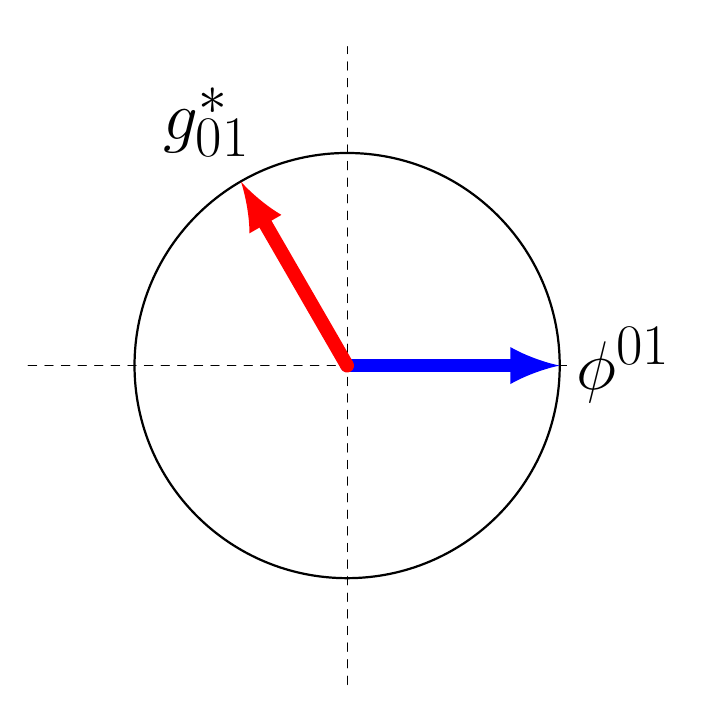
\begin{tikzpicture}[scale=2.7,cap=round,>=latex]
            % draw the coordinates
            \draw[dashed] (-1.5cm,0cm) -- (1.5cm,0cm) node[right,fill=white] {};
            \draw[dashed] (0cm,-1.5cm) -- (0cm,1.5cm) node[above,fill=white] {};
    
            % draw the unit circle
            \draw[thick] (0cm,0cm) circle(1cm);
    
            %phi01
            \draw[blue, ->, line width=5pt] (0cm,0cm) -- (0:1cm);

            %g01
            \draw[red, ->, line width=5pt] (0cm,0cm) -- (120:1cm);

            % text at the end
            \draw (0:1.3cm) node[fill=white, font=\Huge] {$\phi^{01}$};
            \draw (120:1.32cm) node[fill=white, font=\Huge] {$g_{01}^*$};
    
        \end{tikzpicture}}
        \text{\tiny $\boldsymbol{\alpha}$ = 00}
    \end{subfigure}%
    \begin{subfigure}[b]{0.105\textwidth}
        \centering
        \resizebox{\textwidth}{!}{
        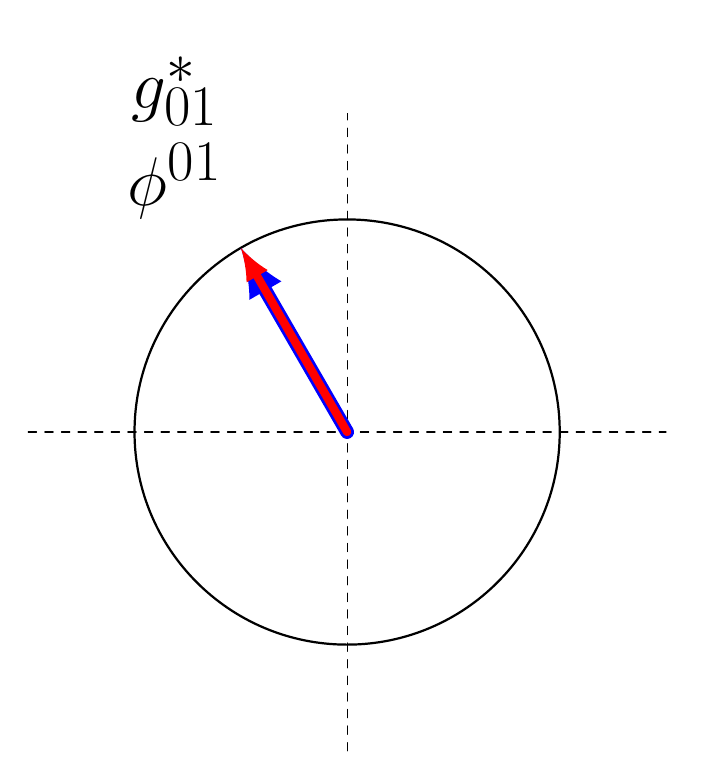
\begin{tikzpicture}[scale=2.7,cap=round,>=latex]
            % draw the coordinates
            \draw[dashed] (-1.5cm,0cm) -- (1.5cm,0cm) node[right,fill=white] {};
            \draw[dashed] (0cm,-1.5cm) -- (0cm,1.5cm) node[above,fill=white] {};
    
            % draw the unit circle
            \draw[thick] (0cm,0cm) circle(1cm);
    
            %phi01
            \draw[blue, ->, line width=5pt] (0cm,0cm) -- (120:1cm);

            %g01
            \draw[red, ->, line width=3pt] (0cm,0cm) -- (120:1cm);

            % text at the end
            \setlength\extrarowheight{5pt}
            \draw (120:1.62cm) node[fill=white, font=\Huge] {\begin{tabular}{c} $g_{01}^*$\\ $\phi^{01}$\end{tabular}};

        \end{tikzpicture}}
        \text{\tiny $\boldsymbol{\alpha}$ = 11}
    \end{subfigure}%
    \begin{subfigure}[b]{0.105\textwidth}
        \centering
        \resizebox{\textwidth}{!}{
        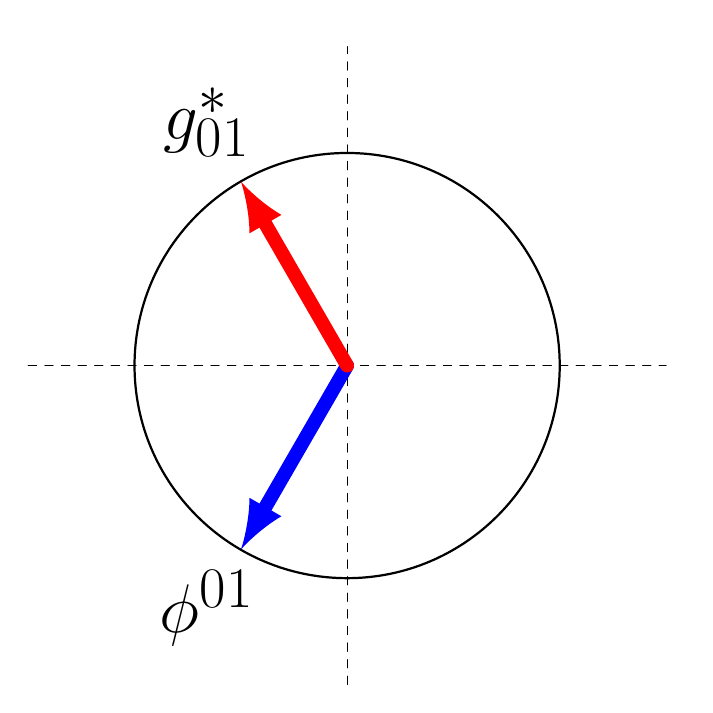
\begin{tikzpicture}[scale=2.7,cap=round,>=latex]
            % draw the coordinates
            \draw[dashed] (-1.5cm,0cm) -- (1.5cm,0cm) node[right,fill=white] {};
            \draw[dashed] (0cm,-1.5cm) -- (0cm,1.5cm) node[above,fill=white] {};
    
            % draw the unit circle
            \draw[thick] (0cm,0cm) circle(1cm);
    
            %phi01
            \draw[blue, ->, line width=5pt] (0cm,0cm) -- (240:1cm);

            %g01
            \draw[red, ->, line width=5pt] (0cm,0cm) -- (120:1cm);

            % text at the end
            \draw (240:1.32cm) node[fill=white, font=\Huge] {$\phi^{01}$};
            \draw (120:1.32cm) node[fill=white, font=\Huge] {$g_{01}^*$};

        \end{tikzpicture}}
        \text{\tiny $\boldsymbol{\alpha}$ = 22}
    \end{subfigure}
    \hfill
    \begin{subfigure}[b]{0.105\textwidth}
        \centering
        \resizebox{\textwidth}{!}{
        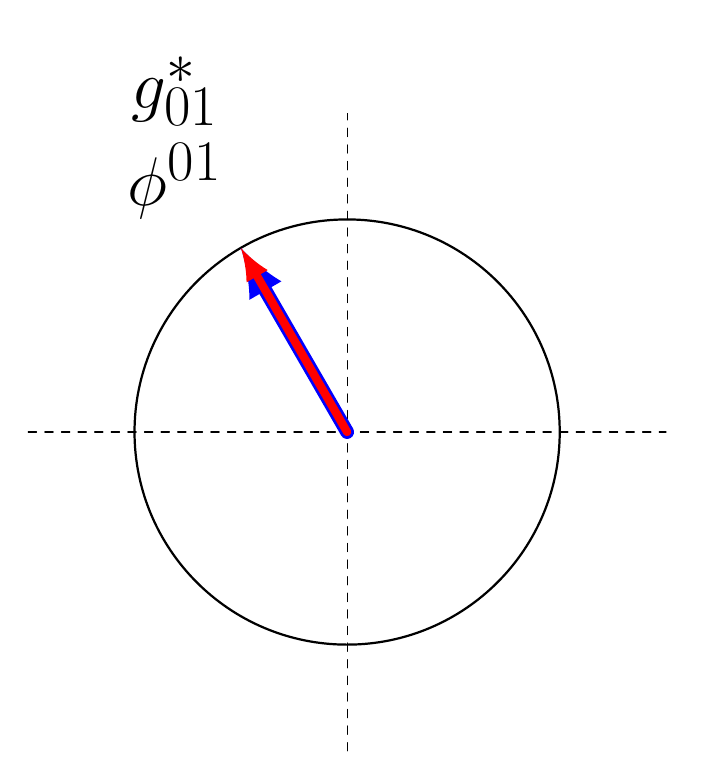
\begin{tikzpicture}[scale=2.7,cap=round,>=latex]
            % draw the coordinates
            \draw[dashed] (-1.5cm,0cm) -- (1.5cm,0cm) node[right,fill=white] {};
            \draw[dashed] (0cm,-1.5cm) -- (0cm,1.5cm) node[above,fill=white] {};
    
            % draw the unit circle
            \draw[thick] (0cm,0cm) circle(1cm);
    
            %phi01
            \draw[blue, ->, line width=5pt] (0cm,0cm) -- (120:1cm);

            %g01
            \draw[red, ->, line width=3pt] (0cm,0cm) -- (120:1cm);

            % text at the end
            \setlength\extrarowheight{5pt}
            \draw (120:1.62cm) node[fill=white, font=\Huge] {\begin{tabular}{c} $g_{01}^*$\\ $\phi^{01}$\end{tabular}};
    
        \end{tikzpicture}}
        \text{\tiny $\boldsymbol{\alpha}$ = 01}
    \end{subfigure}%
    \begin{subfigure}[b]{0.105\textwidth}
        \centering
        \resizebox{\textwidth}{!}{
        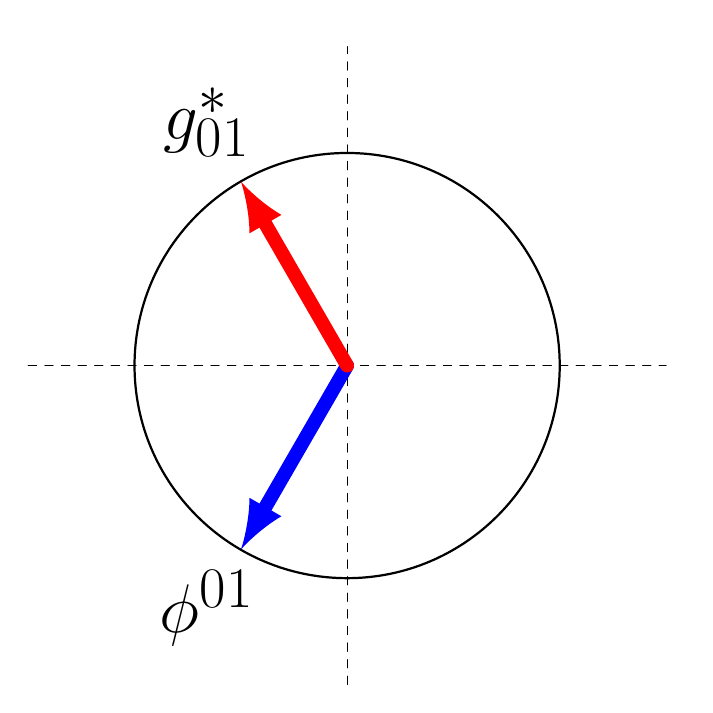
\begin{tikzpicture}[scale=2.7,cap=round,>=latex]
            % draw the coordinates
            \draw[dashed] (-1.5cm,0cm) -- (1.5cm,0cm) node[right,fill=white] {};
            \draw[dashed] (0cm,-1.5cm) -- (0cm,1.5cm) node[above,fill=white] {};
    
            % draw the unit circle
            \draw[thick] (0cm,0cm) circle(1cm);
    
            %phi01
            \draw[blue, ->, line width=5pt] (0cm,0cm) -- (240:1cm);

            %g01
            \draw[red, ->, line width=5pt] (0cm,0cm) -- (120:1cm);

            % text at the end
            \draw (240:1.32cm) node[fill=white, font=\Huge] {$\phi^{01}$};
            \draw (120:1.32cm) node[fill=white, font=\Huge] {$g_{01}^*$};

        \end{tikzpicture}}
        \text{\tiny $\boldsymbol{\alpha}$ = 12}
    \end{subfigure}%
    \begin{subfigure}[b]{0.105\textwidth}
        \centering
        \resizebox{\textwidth}{!}{
        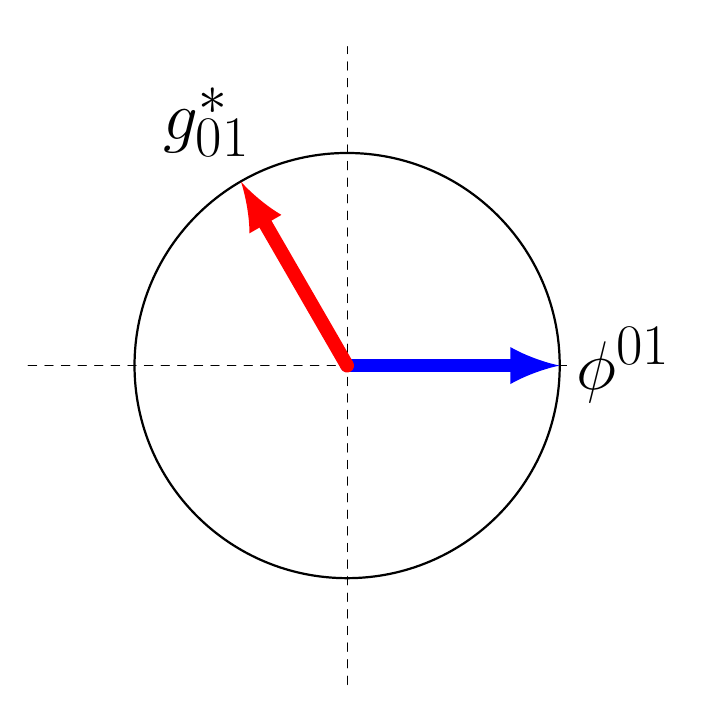
\begin{tikzpicture}[scale=2.7,cap=round,>=latex]
            % draw the coordinates
            \draw[dashed] (-1.5cm,0cm) -- (1.5cm,0cm) node[right,fill=white] {};
            \draw[dashed] (0cm,-1.5cm) -- (0cm,1.5cm) node[above,fill=white] {};
    
            % draw the unit circle
            \draw[thick] (0cm,0cm) circle(1cm);
    
            %phi01
            \draw[blue, ->, line width=5pt] (0cm,0cm) -- (0:1cm);

            %g01
            \draw[red, ->, line width=5pt] (0cm,0cm) -- (120:1cm);

            % text at the end
            \draw (0:1.3cm) node[fill=white, font=\Huge] {$\phi^{01}$};
            \draw (120:1.32cm) node[fill=white, font=\Huge] {$g_{01}^*$};
    
        \end{tikzpicture}}
        \text{\tiny $\boldsymbol{\alpha}$ = 20}
    \end{subfigure}
    \hfill
    \begin{subfigure}[b]{0.105\textwidth}
        \centering
        \resizebox{\textwidth}{!}{
        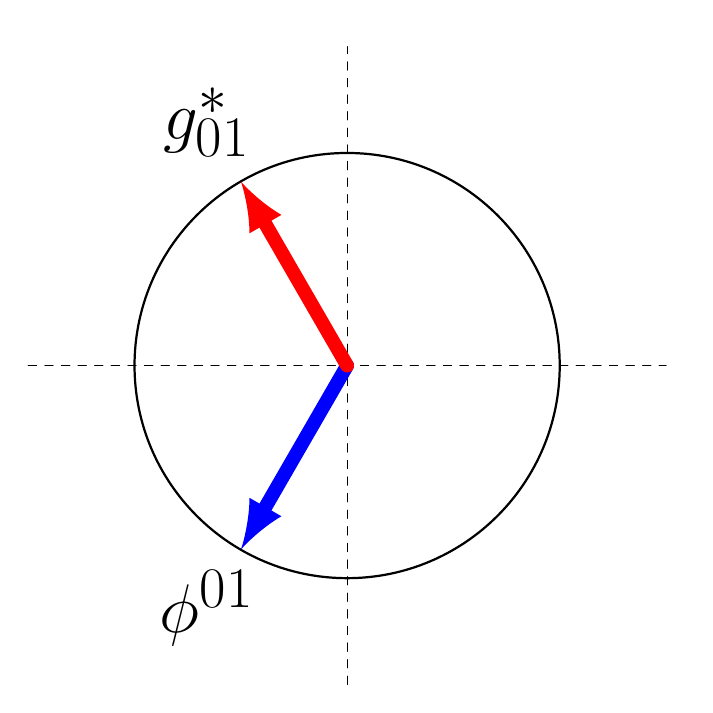
\begin{tikzpicture}[scale=2.7,cap=round,>=latex]
            % draw the coordinates
            \draw[dashed] (-1.5cm,0cm) -- (1.5cm,0cm) node[right,fill=white] {};
            \draw[dashed] (0cm,-1.5cm) -- (0cm,1.5cm) node[above,fill=white] {};
    
            % draw the unit circle
            \draw[thick] (0cm,0cm) circle(1cm);
    
            %phi01
            \draw[blue, ->, line width=5pt] (0cm,0cm) -- (240:1cm);

            %g01
            \draw[red, ->, line width=5pt] (0cm,0cm) -- (120:1cm);

            % text at the end
            \draw (240:1.32cm) node[fill=white, font=\Huge] {$\phi^{01}$};
            \draw (120:1.32cm) node[fill=white, font=\Huge] {$g_{01}^*$};

        \end{tikzpicture}}
        \text{\tiny $\boldsymbol{\alpha}$ = 02}
    \end{subfigure}%
    \begin{subfigure}[b]{0.105\textwidth}
        \centering
        \resizebox{\textwidth}{!}{
        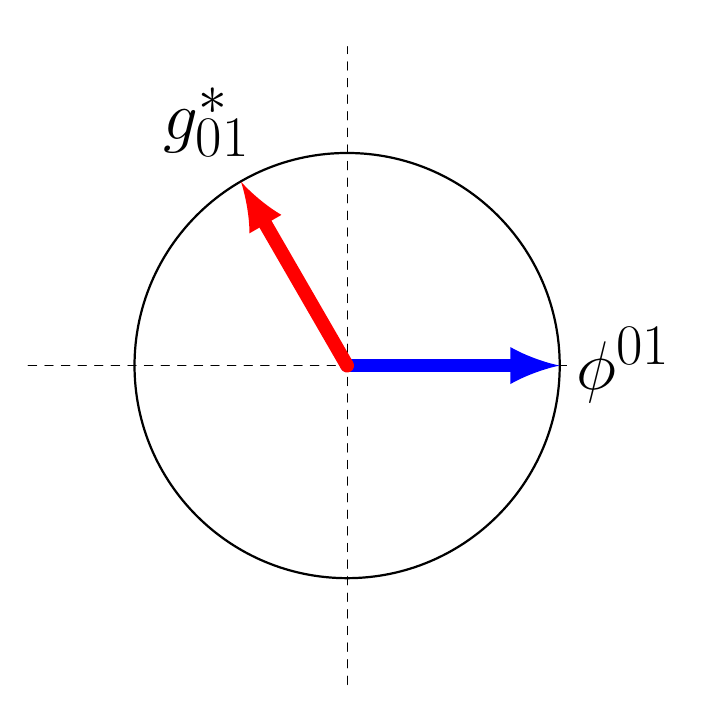
\begin{tikzpicture}[scale=2.7,cap=round,>=latex]
            % draw the coordinates
            \draw[dashed] (-1.5cm,0cm) -- (1.5cm,0cm) node[right,fill=white] {};
            \draw[dashed] (0cm,-1.5cm) -- (0cm,1.5cm) node[above,fill=white] {};
    
            % draw the unit circle
            \draw[thick] (0cm,0cm) circle(1cm);
    
            %phi01
            \draw[blue, ->, line width=5pt] (0cm,0cm) -- (0:1cm);

            %g01
            \draw[red, ->, line width=5pt] (0cm,0cm) -- (120:1cm);

            % text at the end
            \draw (0:1.3cm) node[fill=white, font=\Huge] {$\phi^{01}$};
            \draw (120:1.32cm) node[fill=white, font=\Huge] {$g_{01}^*$};
    
        \end{tikzpicture}}
        \text{\tiny $\boldsymbol{\alpha}$ = 10}
    \end{subfigure}%
    \begin{subfigure}[b]{0.105\textwidth}
        \centering
        \resizebox{\textwidth}{!}{
        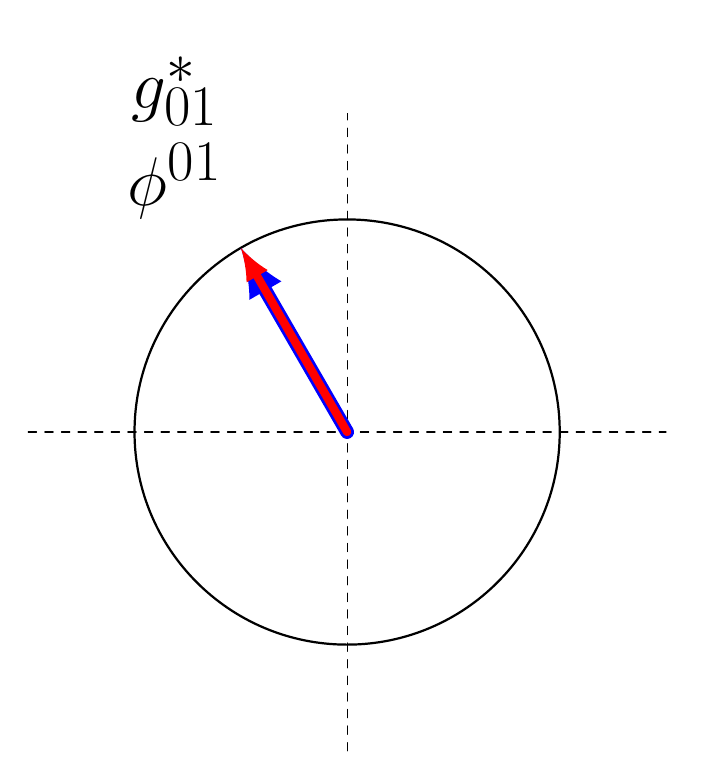
\begin{tikzpicture}[scale=2.7,cap=round,>=latex]
            % draw the coordinates
            \draw[dashed] (-1.5cm,0cm) -- (1.5cm,0cm) node[right,fill=white] {};
            \draw[dashed] (0cm,-1.5cm) -- (0cm,1.5cm) node[above,fill=white] {};
    
            % draw the unit circle
            \draw[thick] (0cm,0cm) circle(1cm);
    
            %phi01
            \draw[blue, ->, line width=5pt] (0cm,0cm) -- (120:1cm);

            %g01
            \draw[red, ->, line width=3pt] (0cm,0cm) -- (120:1cm);

            % text at the end
            \setlength\extrarowheight{5pt}
            \draw (120:1.62cm) node[fill=white, font=\Huge] {\begin{tabular}{c} $g_{01}^*$\\ $\phi^{01}$\end{tabular}};

        \end{tikzpicture}}
        \text{\tiny $\boldsymbol{\alpha}$ = 21}
    \end{subfigure}%
    \caption{Graphical representation of $S({\boldsymbol{\alpha}})$ of a 3-state,2-spin system with a first-order interaction, $\phi^{01}$ and $\phi^{01}$, and a second order interaction, $\phi^{12}$ and $\phi^{21}$. The parameters for the first-order interaction are chosen such that states where $\alpha_2 = 1$ are preferred and the parameters of the second-order interactions such that states for which  $\sum_{j \in \mu} \alpha_j \mu_j =  0\mod3$ are preferred.}
    \label{fig:s_case_2}
\end{figure}

\begin{table}[h]
    \centering
    \caption{Numerical values for S($\boldsymbol{\alpha}$) and P($\boldsymbol{\alpha}$) for a spin model with a first-order interaction, $\phi^{01}$ and $\phi^{01}$, and a second order interaction, $\phi^{12}$ and $\phi^{21}$.}
    \label{tab:case_2_num_values}
    \begin{subtable}{.3\textwidth}
        \centering
        \caption{r = 0.5}
        \begin{tabular}{ccc}
            \toprule
             $\boldsymbol{\alpha}$ & S($\boldsymbol{\alpha}$) & P($\boldsymbol{\alpha}$)\\
            \midrule
            00 & 0.5 & 0.107 \\
            01 & 0.5 & 0.107 \\
            02 & -1 & 0.024 \\
            10 & -1 & 0.024 \\
            11 & 2 & 0.478 \\
            12 & -1 & 0.024 \\
            20 & -1 & 0.024 \\
            21 & 0.5 & 0.107 \\
            22 & 0.5 & 0.107\\
          \bottomrule
        \end{tabular}
    \end{subtable}%
    \begin{subtable}{.3\textwidth}
        \centering
        \caption{r = 1}
        \begin{tabular}{ccc}
            \toprule
             $\boldsymbol{\alpha}$ & S($\boldsymbol{\alpha}$) & P($\boldsymbol{\alpha}$)\\
            \midrule
            00 & 1 & 0.041 \\
            01 & 1 & 0.041 \\
            02 & -2 & 0.002 \\
            10 & -2 & 0.002 \\
            11 & 4 & 0.827 \\
            12 & -2 & 0.002 \\
            20 & -2 & 0.002 \\
            21 & 1 & 0.041 \\
            22 & 1 & 0.041 \\
          \bottomrule
        \end{tabular}
    \end{subtable}%
    \begin{subtable}{.3\textwidth}
        \centering
        \caption{r = 2}
        \begin{tabular}{ccc}
            \toprule
             $\boldsymbol{\alpha}$ & S($\boldsymbol{\alpha}$) & P($\boldsymbol{\alpha}$)\\
            \midrule
            00 & 2 & 0.002 \\
            01 & 2 & 0.002 \\
            02 & -4 & 0.000 \\
            10 & -4 & 0.000 \\
            11 & 8 & 0.990 \\
            12 & -4 & 0.000 \\
            20 & -4 & 0.000 \\
            21 & 2 & 0.002 \\
            22 & 2 & 0.002 \\
          \bottomrule
        \end{tabular}
    \end{subtable}
\end{table}

\noindent
\textit{Case 3: Two second-order interactions}

\begin{itemize}
    \item $g_{11}$ = $r\left[\cos\left( \frac{4\pi}{3}\right) + i \sin\left( \frac{4\pi}{3}\right)\right]$
    \item $g_{22}$ = $r\left[\cos\left( \frac{4\pi}{3}\right) - i \sin\left( \frac{4\pi}{3}\right)\right]$
    \item $g_{12}$ = $r$
    \item $g_{21}$ = $r$
\end{itemize}

\begin{figure}[h!]
    \centering
    \begin{subfigure}[b]{0.33\textwidth}
        \centering
        \resizebox{\textwidth}{!}{
        \begin{tikzpicture}[scale=2.7,cap=round,>=latex]
            % draw the coordinates
            \draw[dashed] (-1.5cm,0cm) -- (1.5cm,0cm) node[right,fill=white] {};
            \draw[dashed] (0cm,-1.5cm) -- (0cm,1.5cm) node[above,fill=white] {};
    
            % draw the unit circle
            \draw[thick] (0cm,0cm) circle(1cm);
    
            %phi12
            \draw[blue, ->, ultra thick] (0cm,0cm) -- (0:1cm);

            %g12
            \draw[red, ->, thick] (0cm,0cm) -- (0:1cm);

            %projection
            \filldraw[black] (0:1cm) circle(0.6pt);

            % text at the end
            \draw (0:1.25cm) node[fill=white] {\begin{tabular}{c} $g_{12}^*$\\$\phi^{12}$\end{tabular}};
    
            % draw the horizontal and vertical coordinates
            \draw (1.45cm,0cm)  node[above=1pt] {$\Re$}
                (0cm,1.4cm)  node[fill=white] {$\Im$};
        \end{tikzpicture}}
    \end{subfigure}%
    \begin{subfigure}[b]{0.33\textwidth}
        \centering
        \resizebox{\textwidth}{!}{
        \begin{tikzpicture}[scale=2.7,cap=round,>=latex]
            % draw the coordinates
            \draw[dashed] (-1.5cm,0cm) -- (1.5cm,0cm) node[right,fill=white] {};
            \draw[dashed] (0cm,-1.5cm) -- (0cm,1.5cm) node[above,fill=white] {};
    
            % draw the unit circle
            \draw[thick] (0cm,0cm) circle(1cm);
    
            %phi12
            \draw[blue, ->, ultra thick] (0cm,0cm) -- (240:1cm);

            %g12
            \draw[red, ->, ultra thick] (0cm,0cm) -- (0:1cm);

            %projection
            \draw[dashdotted] (0:1cm) -- (60:.5cm);
            \filldraw[black] (60:.5cm) circle(0.6pt);

            % text at the end
            \draw (240:1.3cm) node[fill=white] {\begin{tabular}{c} $\phi^{12}$\end{tabular}};
            \draw (0:1.15cm) node[fill=white] {$g_{12}^*$};
        
            % draw the horizontal and vertical coordinates
            \draw (1.4cm,0cm)  node[above=1pt] {$\Re$}
                (0cm,1.4cm)  node[fill=white] {$\Im$};
        \end{tikzpicture}}
    \end{subfigure}%
    \begin{subfigure}[b]{0.33\textwidth}
        \centering
        \resizebox{\textwidth}{!}{
        \begin{tikzpicture}[scale=2.7,cap=round,>=latex]
            % draw the coordinates
            \draw[dashed] (-1.5cm,0cm) -- (1.5cm,0cm) node[right,fill=white] {};
            \draw[dashed] (0cm,-1.5cm) -- (0cm,1.5cm) node[above,fill=white] {};
    
            % draw the unit circle
            \draw[thick] (0cm,0cm) circle(1cm);
        
            %phi12
            \draw[blue, ->, ultra thick] (0cm,0cm) -- (120:1cm);

            %g12
            \draw[red, ->, ultra thick] (0cm,0cm) -- (0:1cm);

            %projection
            \draw[dashdotted] (0:1cm) -- (300:.5cm);
            \filldraw[black] (300:.5cm) circle(0.6pt);

            % text at the end
            \draw (120:1.3cm) node[fill=white] {\begin{tabular}{c} $\phi^{12}$\end{tabular}};
            \draw (0:1.15cm) node[fill=white] {$g_{12}^*$};
        
            % draw the horizontal and vertical coordinates
            \draw (1.5cm,0cm)  node[above=1pt] {$\Re$}
                (0cm,1.4cm)  node[fill=white] {$\Im$};
        \end{tikzpicture}}
    \end{subfigure}
    \begin{subfigure}[b]{0.105\textwidth}
        \centering
        \resizebox{\textwidth}{!}{
        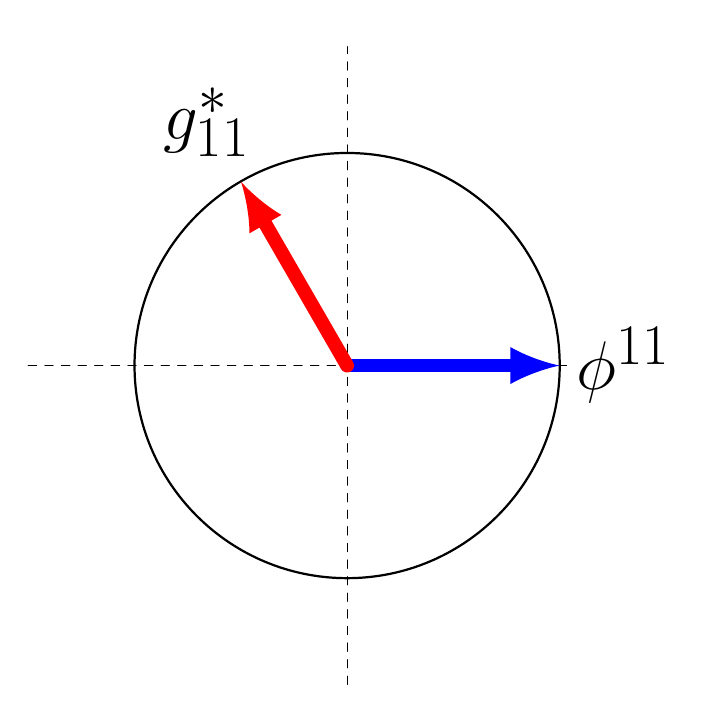
\begin{tikzpicture}[scale=2.7,cap=round,>=latex]
            % draw the coordinates
            \draw[dashed] (-1.5cm,0cm) -- (1.5cm,0cm) node[right,fill=white] {};
            \draw[dashed] (0cm,-1.5cm) -- (0cm,1.5cm) node[above,fill=white] {};
    
            % draw the unit circle
            \draw[thick] (0cm,0cm) circle(1cm);
    
            %phi11
            \draw[blue, ->, line width=5pt] (0cm,0cm) -- (0:1cm);

            %g11
            \draw[red, ->, line width=5pt] (0cm,0cm) -- (120:1cm);

            % text at the end
            \draw (0:1.3cm) node[fill=white, font=\Huge] {$\phi^{11}$};
            \draw (120:1.32cm) node[fill=white, font=\Huge] {$g_{11}^*$};
    
        \end{tikzpicture}}
        \text{\tiny $\boldsymbol{\alpha}$ = 00}
    \end{subfigure}%
    \begin{subfigure}[b]{0.105\textwidth}
        \centering
        \resizebox{\textwidth}{!}{
        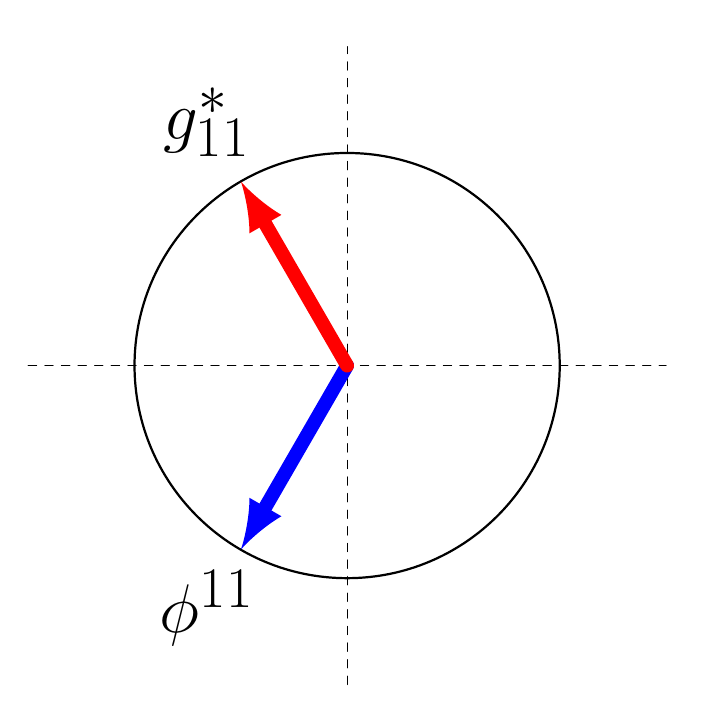
\begin{tikzpicture}[scale=2.7,cap=round,>=latex]
            % draw the coordinates
            \draw[dashed] (-1.5cm,0cm) -- (1.5cm,0cm) node[right,fill=white] {};
            \draw[dashed] (0cm,-1.5cm) -- (0cm,1.5cm) node[above,fill=white] {};
    
            % draw the unit circle
            \draw[thick] (0cm,0cm) circle(1cm);
    
            %phi11
            \draw[blue, ->, line width=5pt] (0cm,0cm) -- (240:1cm);

            %g11
            \draw[red, ->, line width=5pt] (0cm,0cm) -- (120:1cm);

            % text at the end
            \draw (240:1.32cm) node[fill=white, font=\Huge] {$\phi^{11}$};
            \draw (120:1.32cm) node[fill=white, font=\Huge] {$g_{11}^*$};
    
        \end{tikzpicture}}
        \text{\tiny $\boldsymbol{\alpha}$ = 11}
    \end{subfigure}%
    \begin{subfigure}[b]{0.105\textwidth}
        \centering
        \resizebox{\textwidth}{!}{
        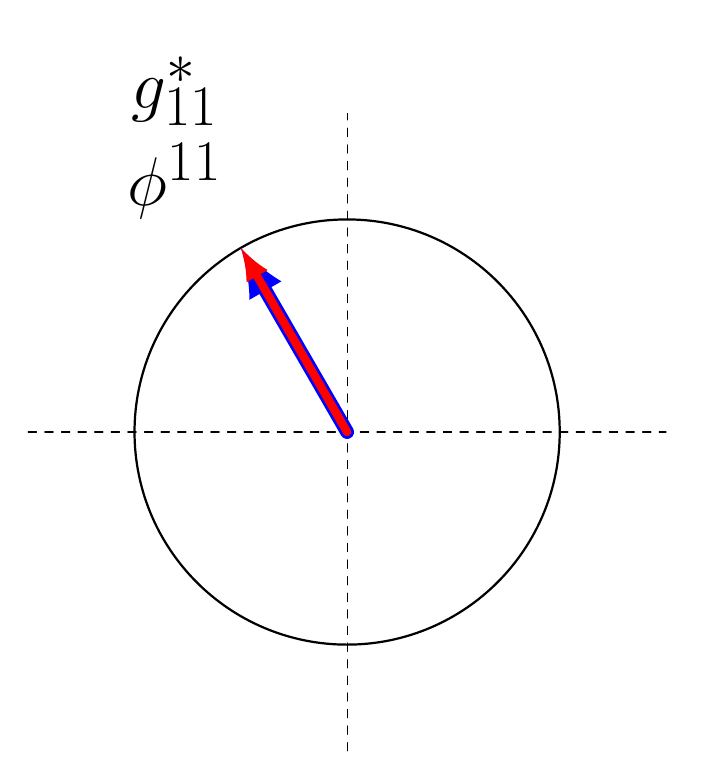
\begin{tikzpicture}[scale=2.7,cap=round,>=latex]
            % draw the coordinates
            \draw[dashed] (-1.5cm,0cm) -- (1.5cm,0cm) node[right,fill=white] {};
            \draw[dashed] (0cm,-1.5cm) -- (0cm,1.5cm) node[above,fill=white] {};
    
            % draw the unit circle
            \draw[thick] (0cm,0cm) circle(1cm);
    
            %phi11
            \draw[blue, ->, line width=5pt] (0cm,0cm) -- (120:1cm);

            %g11
            \draw[red, ->, line width=3pt] (0cm,0cm) -- (120:1cm);

            % text at the end
            \setlength\extrarowheight{5pt}
            \draw (120:1.62cm) node[fill=white, font=\Huge] {\begin{tabular}{c} $g_{11}^*$\\ $\phi^{11}$\end{tabular}};

        \end{tikzpicture}}
        \text{\tiny $\boldsymbol{\alpha}$ = 22}
    \end{subfigure}
    \hfill
    \begin{subfigure}[b]{0.105\textwidth}
        \centering
        \resizebox{\textwidth}{!}{
        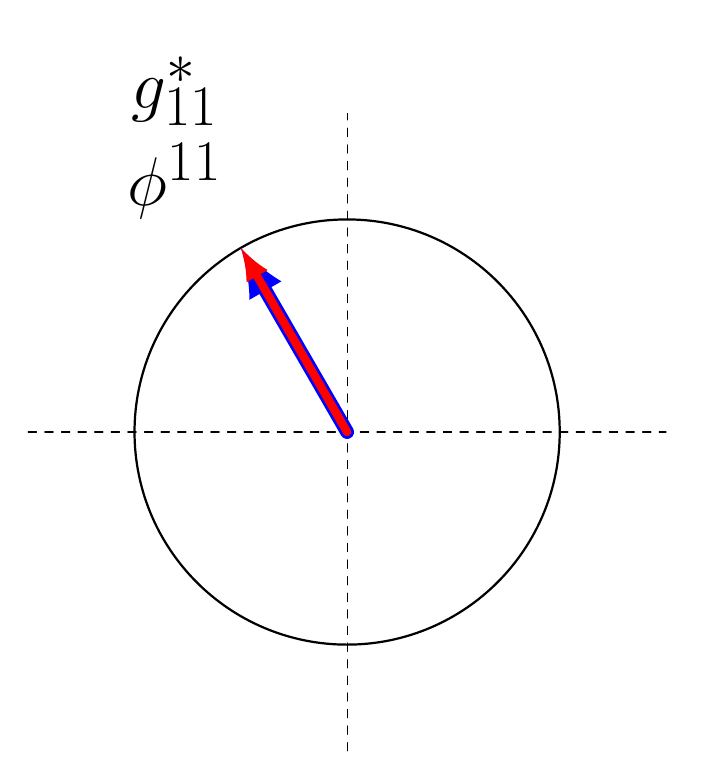
\begin{tikzpicture}[scale=2.7,cap=round,>=latex]
            % draw the coordinates
            \draw[dashed] (-1.5cm,0cm) -- (1.5cm,0cm) node[right,fill=white] {};
            \draw[dashed] (0cm,-1.5cm) -- (0cm,1.5cm) node[above,fill=white] {};
    
            % draw the unit circle
            \draw[thick] (0cm,0cm) circle(1cm);
    
            %phi11
            \draw[blue, ->, line width=5pt] (0cm,0cm) -- (120:1cm);

            %g11
            \draw[red, ->, line width=3pt] (0cm,0cm) -- (120:1cm);

            % text at the end
            \setlength\extrarowheight{5pt}
            \draw (120:1.62cm) node[fill=white, font=\Huge] {\begin{tabular}{c} $g_{11}^*$\\ $\phi^{11}$\end{tabular}};

        \end{tikzpicture}}
        \text{\tiny $\boldsymbol{\alpha}$ = 01}
    \end{subfigure}%
    \begin{subfigure}[b]{0.105\textwidth}
        \centering
        \resizebox{\textwidth}{!}{
        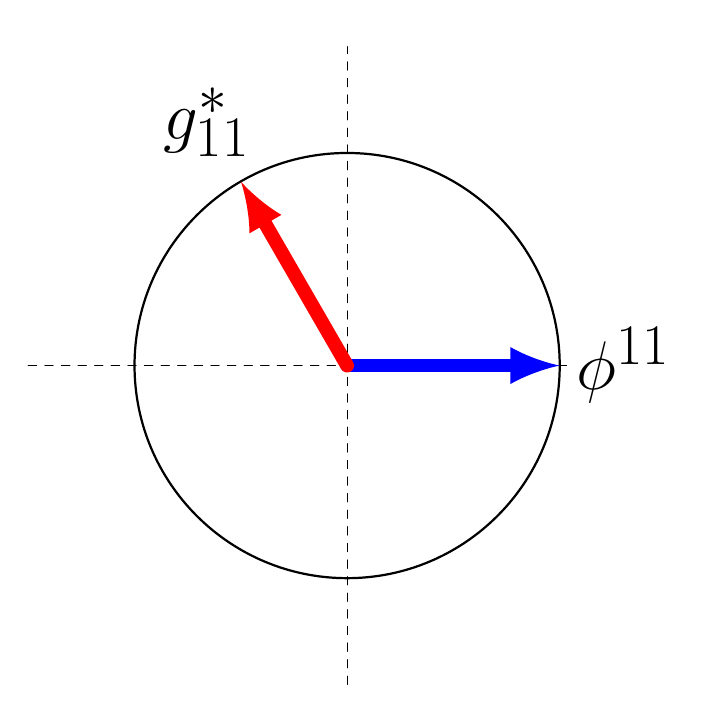
\begin{tikzpicture}[scale=2.7,cap=round,>=latex]
            % draw the coordinates
            \draw[dashed] (-1.5cm,0cm) -- (1.5cm,0cm) node[right,fill=white] {};
            \draw[dashed] (0cm,-1.5cm) -- (0cm,1.5cm) node[above,fill=white] {};
    
            % draw the unit circle
            \draw[thick] (0cm,0cm) circle(1cm);
    
            %phi11
            \draw[blue, ->, line width=5pt] (0cm,0cm) -- (0:1cm);

            %g11
            \draw[red, ->, line width=5pt] (0cm,0cm) -- (120:1cm);

            % text at the end
            \draw (0:1.3cm) node[fill=white, font=\Huge] {$\phi^{11}$};
            \draw (120:1.32cm) node[fill=white, font=\Huge] {$g_{11}^*$};
    
        \end{tikzpicture}}
        \text{\tiny $\boldsymbol{\alpha}$ = 12}
    \end{subfigure}%
    \begin{subfigure}[b]{0.105\textwidth}
        \centering
        \resizebox{\textwidth}{!}{
        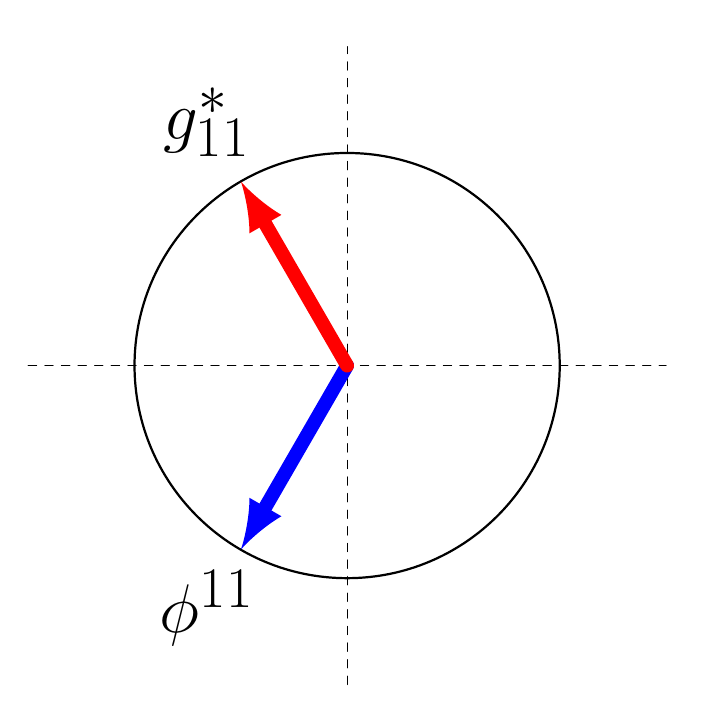
\begin{tikzpicture}[scale=2.7,cap=round,>=latex]
            % draw the coordinates
            \draw[dashed] (-1.5cm,0cm) -- (1.5cm,0cm) node[right,fill=white] {};
            \draw[dashed] (0cm,-1.5cm) -- (0cm,1.5cm) node[above,fill=white] {};
    
            % draw the unit circle
            \draw[thick] (0cm,0cm) circle(1cm);
    
            %phi11
            \draw[blue, ->, line width=5pt] (0cm,0cm) -- (240:1cm);

            %g11
            \draw[red, ->, line width=5pt] (0cm,0cm) -- (120:1cm);

            % text at the end
            \draw (240:1.32cm) node[fill=white, font=\Huge] {$\phi^{11}$};
            \draw (120:1.32cm) node[fill=white, font=\Huge] {$g_{11}^*$};
    
        \end{tikzpicture}}
        \text{\tiny $\boldsymbol{\alpha}$ = 20}
    \end{subfigure}
    \hfill
    \begin{subfigure}[b]{0.105\textwidth}
        \centering
        \resizebox{\textwidth}{!}{
        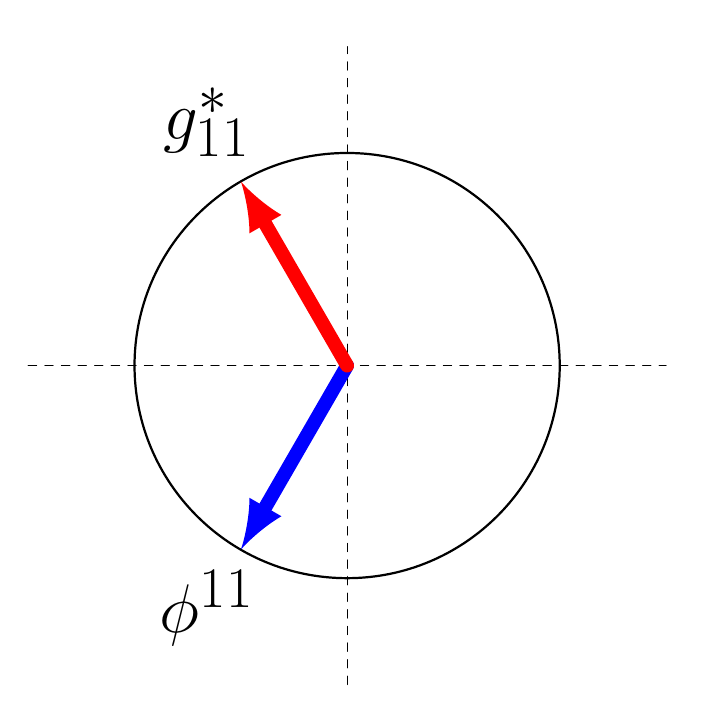
\begin{tikzpicture}[scale=2.7,cap=round,>=latex]
            % draw the coordinates
            \draw[dashed] (-1.5cm,0cm) -- (1.5cm,0cm) node[right,fill=white] {};
            \draw[dashed] (0cm,-1.5cm) -- (0cm,1.5cm) node[above,fill=white] {};
    
            % draw the unit circle
            \draw[thick] (0cm,0cm) circle(1cm);
    
            %phi11
            \draw[blue, ->, line width=5pt] (0cm,0cm) -- (240:1cm);

            %g11
            \draw[red, ->, line width=5pt] (0cm,0cm) -- (120:1cm);

            % text at the end
            \draw (240:1.32cm) node[fill=white, font=\Huge] {$\phi^{11}$};
            \draw (120:1.32cm) node[fill=white, font=\Huge] {$g_{11}^*$};
    
        \end{tikzpicture}}
        \text{\tiny $\boldsymbol{\alpha}$ = 02}
    \end{subfigure}%
    \begin{subfigure}[b]{0.105\textwidth}
        \centering
        \resizebox{\textwidth}{!}{
        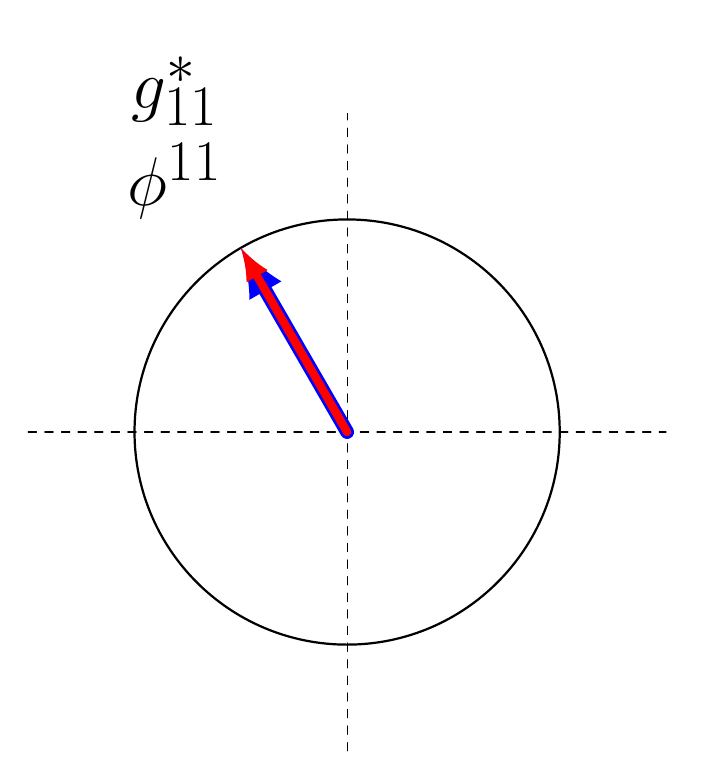
\begin{tikzpicture}[scale=2.7,cap=round,>=latex]
            % draw the coordinates
            \draw[dashed] (-1.5cm,0cm) -- (1.5cm,0cm) node[right,fill=white] {};
            \draw[dashed] (0cm,-1.5cm) -- (0cm,1.5cm) node[above,fill=white] {};
    
            % draw the unit circle
            \draw[thick] (0cm,0cm) circle(1cm);
    
            %phi11
            \draw[blue, ->, line width=5pt] (0cm,0cm) -- (120:1cm);

            %g11
            \draw[red, ->, line width=3pt] (0cm,0cm) -- (120:1cm);

            % text at the end
            \setlength\extrarowheight{5pt}
            \draw (120:1.62cm) node[fill=white, font=\Huge] {\begin{tabular}{c} $g_{11}^*$\\ $\phi^{11}$\end{tabular}};

        \end{tikzpicture}}
        \text{\tiny $\boldsymbol{\alpha}$ = 10}
    \end{subfigure}%
    \begin{subfigure}[b]{0.105\textwidth}
        \centering
        \resizebox{\textwidth}{!}{
        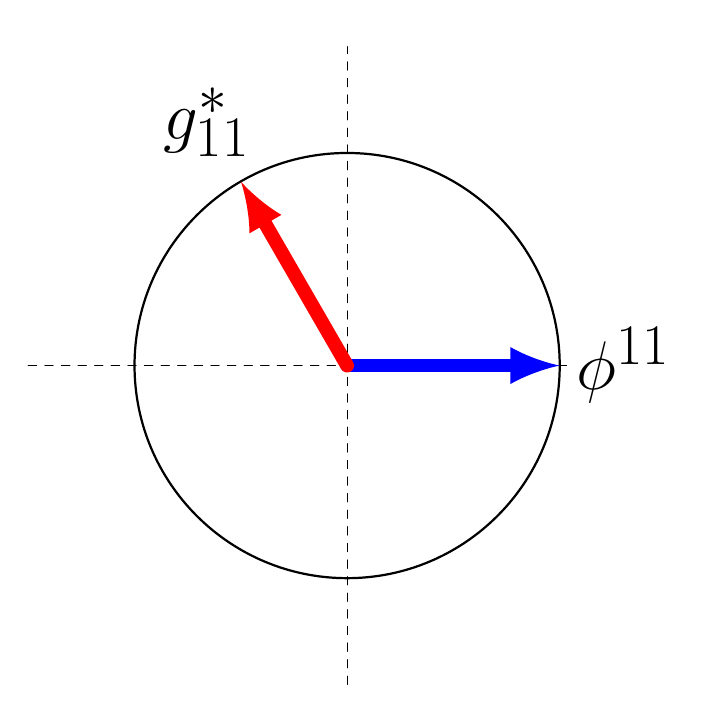
\begin{tikzpicture}[scale=2.7,cap=round,>=latex]
            % draw the coordinates
            \draw[dashed] (-1.5cm,0cm) -- (1.5cm,0cm) node[right,fill=white] {};
            \draw[dashed] (0cm,-1.5cm) -- (0cm,1.5cm) node[above,fill=white] {};
    
            % draw the unit circle
            \draw[thick] (0cm,0cm) circle(1cm);
    
            %phi11
            \draw[blue, ->, line width=5pt] (0cm,0cm) -- (0:1cm);

            %g11
            \draw[red, ->, line width=5pt] (0cm,0cm) -- (120:1cm);

            % text at the end
            \draw (0:1.3cm) node[fill=white, font=\Huge] {$\phi^{11}$};
            \draw (120:1.32cm) node[fill=white, font=\Huge] {$g_{11}^*$};
    
        \end{tikzpicture}}
        \text{\tiny $\boldsymbol{\alpha}$ = 21}
    \end{subfigure}%
    \caption{Graphical representation of $S({\boldsymbol{\alpha}})$ of a 3-state,2-spin system with two second order interactions. 
    The parameter $g_{12}$ is chosen such that states for which  $\sum_{j \in \mu} \alpha_j \mu_j =  0\mod3$ are preferred and the parameter $g_{11}$ is chosen such that states for which  $\sum_{j \in \mu} \alpha_j \mu_j =  1\mod3$ are preferred.}
    \label{fig:s_case_3}
\end{figure}

\begin{table}[h]
    \centering
    \caption{Numerical values for S($\boldsymbol{\alpha}$) and P($\boldsymbol{\alpha}$) for a spin model with two second order interactions.}
    \label{tab:case_2_num_values}
    \begin{subtable}{.3\textwidth}
        \centering
        \caption{r = 0.5}
        \begin{tabular}{ccc}
            \toprule
             $\boldsymbol{\alpha}$ & S($\boldsymbol{\alpha}$) & P($\boldsymbol{\alpha}$)\\
            \midrule
            00 & 0.5 & 0.107 \\
            01 & 0.5 & 0.107 \\
            02 & -1 & 0.024 \\
            10 & -1 & 0.024 \\
            11 & 2 & 0.478 \\
            12 & -1 & 0.024 \\
            20 & -1 & 0.024 \\
            21 & 0.5 & 0.107 \\
            22 & 0.5 & 0.107\\
          \bottomrule
        \end{tabular}
    \end{subtable}%
    \begin{subtable}{.3\textwidth}
        \centering
        \caption{r = 1}
        \begin{tabular}{ccc}
            \toprule
             $\boldsymbol{\alpha}$ & S($\boldsymbol{\alpha}$) & P($\boldsymbol{\alpha}$)\\
            \midrule
            00 & 1 & 0.041 \\
            01 & 1 & 0.041 \\
            02 & -2 & 0.002 \\
            10 & -2 & 0.002 \\
            11 & 4 & 0.827 \\
            12 & -2 & 0.002 \\
            20 & -2 & 0.002 \\
            21 & 1 & 0.041 \\
            22 & 1 & 0.041 \\
          \bottomrule
        \end{tabular}
    \end{subtable}%
    \begin{subtable}{.3\textwidth}
        \centering
        \caption{r = 2}
        \begin{tabular}{ccc}
            \toprule
             $\boldsymbol{\alpha}$ & S($\boldsymbol{\alpha}$) & P($\boldsymbol{\alpha}$)\\
            \midrule
            00 & 2 & 0.002 \\
            01 & 2 & 0.002 \\
            02 & -4 & 0.000 \\
            10 & -4 & 0.000 \\
            11 & 8 & 0.990 \\
            12 & -4 & 0.000 \\
            20 & -4 & 0.000 \\
            21 & 2 & 0.002 \\
            22 & 2 & 0.002 \\
          \bottomrule
        \end{tabular}
    \end{subtable}
\end{table}